\chapter{ReceiptBudget: A System for Managing Personal Finances Based on Receipts}
\label{chap:application}

% ii ok o introducere asa personala?
The idea for ReceiptBudget came out of a necessity most students face when they come to college and have to manage their own money for the first time. They are most often overspending and not keeping good track of their finances. Most existing tools are difficult to use or require a lot of time. Some try to use Excel spreadsheets to record their expenses, but that is tedious and easy to forget to do. Others, like Mint \cite{mint}, that offered very detailed reports and forecasts, would get the information by linking to a bank account. GnuCash \cite{gnucash}, had an extremely complicated system for doing double bookkeeping. Programs like Toshl \cite{toshl} or ExpenseIQ \cite{expenseiq} weren't doing much more than an Excel spreadsheet with a couple of charts, and entering data is not any easier. 

ReceiptBudget is a solution to all these problems and to help people manage their budgets, presented in this thesis. It is  really easy to add expenses by taking a photo of a receipt and having the OCR engine extract the details from the photo. There would have to be lots of reports, which can be filtered by months, shops or items, so that the users could observe spending patterns and hopefully do something about them.

\section{The OCR Engine. Our proposal}
The OCR engine does three things: it preprocesses and normalizes an image containing a receipt, it recognizes the text that is written on each line and then it extracts useful information from that text. 

\subsection{Model design}

\subsubsection{The Random Forest Model}
The random forest was used as a model for the character segmentation problem. The criterion for choosing the best feature to split a node is the information gain (entropy). Trees are grown to their full depth, no pruning or limitation is applied to the branches. 

The other parameters of the random forest were chosen by cross-validation: the number of trees and the number of features to consider when randomly sampling from the feature space. 

\subsubsection{The Support Vector Machine Model}
The SVM was used as a baseline for the character recognition problem. The performance of both linear and radial basis function kernels was evaluated. 

The regularization parameter of the SVM was determined using cross-validation. 

\subsubsection{The Neural Network Model}
Neural networks were used for recognizing the characters. Various models were tried, including Autoencoders, Rectified Linear Units and Dropout. 


\subsection{Document Layout Analysis}
Before any characters can be recognized in a receipt, the image must first be preprocessed and normalized. This is done in several steps. 

The preprocessing consists of binarizing the images, using Otsu's method\cite{otsu1975threshold}, which adapts the threshold based on the histogram of the image. This step is done to remove any noise and speckles from the image. The result of this operation is seen in Figure \ref{fig:bin_image}.

The first step in normalization is to straighten the images. The receipts are assumed to be photographed with a mobile phone camera. Users will most often take photos that are slightly rotated. The orientation of the images is assumed to be vertical, so the software will not try to identify if the receipt is horizontal. To straighten the images, they are rotated from -10 to 10 degrees, with a 0.3 angle step, and a horizontal projection (summing the pixel values row-wise) is done for each resulting image. The straight image is assumed to be the one with the highest peak in the histogram, because in the straight image there would be many pixel-wise line that have the same amount of color on them, while on crooked images, the pixel count of each line would be distributed more uniformly. An example of such a histogram can be seen in Figure \ref{fig:hist_plot}. The straightened image can be seen in Figure \ref{fig:straight_image}.

The following step is removing the edges of the image, to keep only the receipt, removing any background. Due to variations in illumination, we cannot simply look for white patches to identify the receipt, because mobile cameras often use flash which gives receipts a blue tint while photos taken indoor close to a source of light have a yellow hue. The approach that was used was to look at the horizontal projections and to remove the section from the left and right that is over a threshold. An example of such a projection can be seen in Figure \ref{fig:edge_plot}. This final version of the image is seen in Figure \ref{fig:edge_image}.

The last step is detecting the lines in the receipt. Because the images are already straight and without edges, all we have to do is identify the peaks in the horizontal histogram in the image. These peaks can be easily seen in Figure \ref{fig:line_plot}. Some of the extracted lines can be seen in Figure \ref{fig:line_samples}.


\begin{figure}
\centering
\begin{subfigure}{0.49\linewidth}
  \centering
  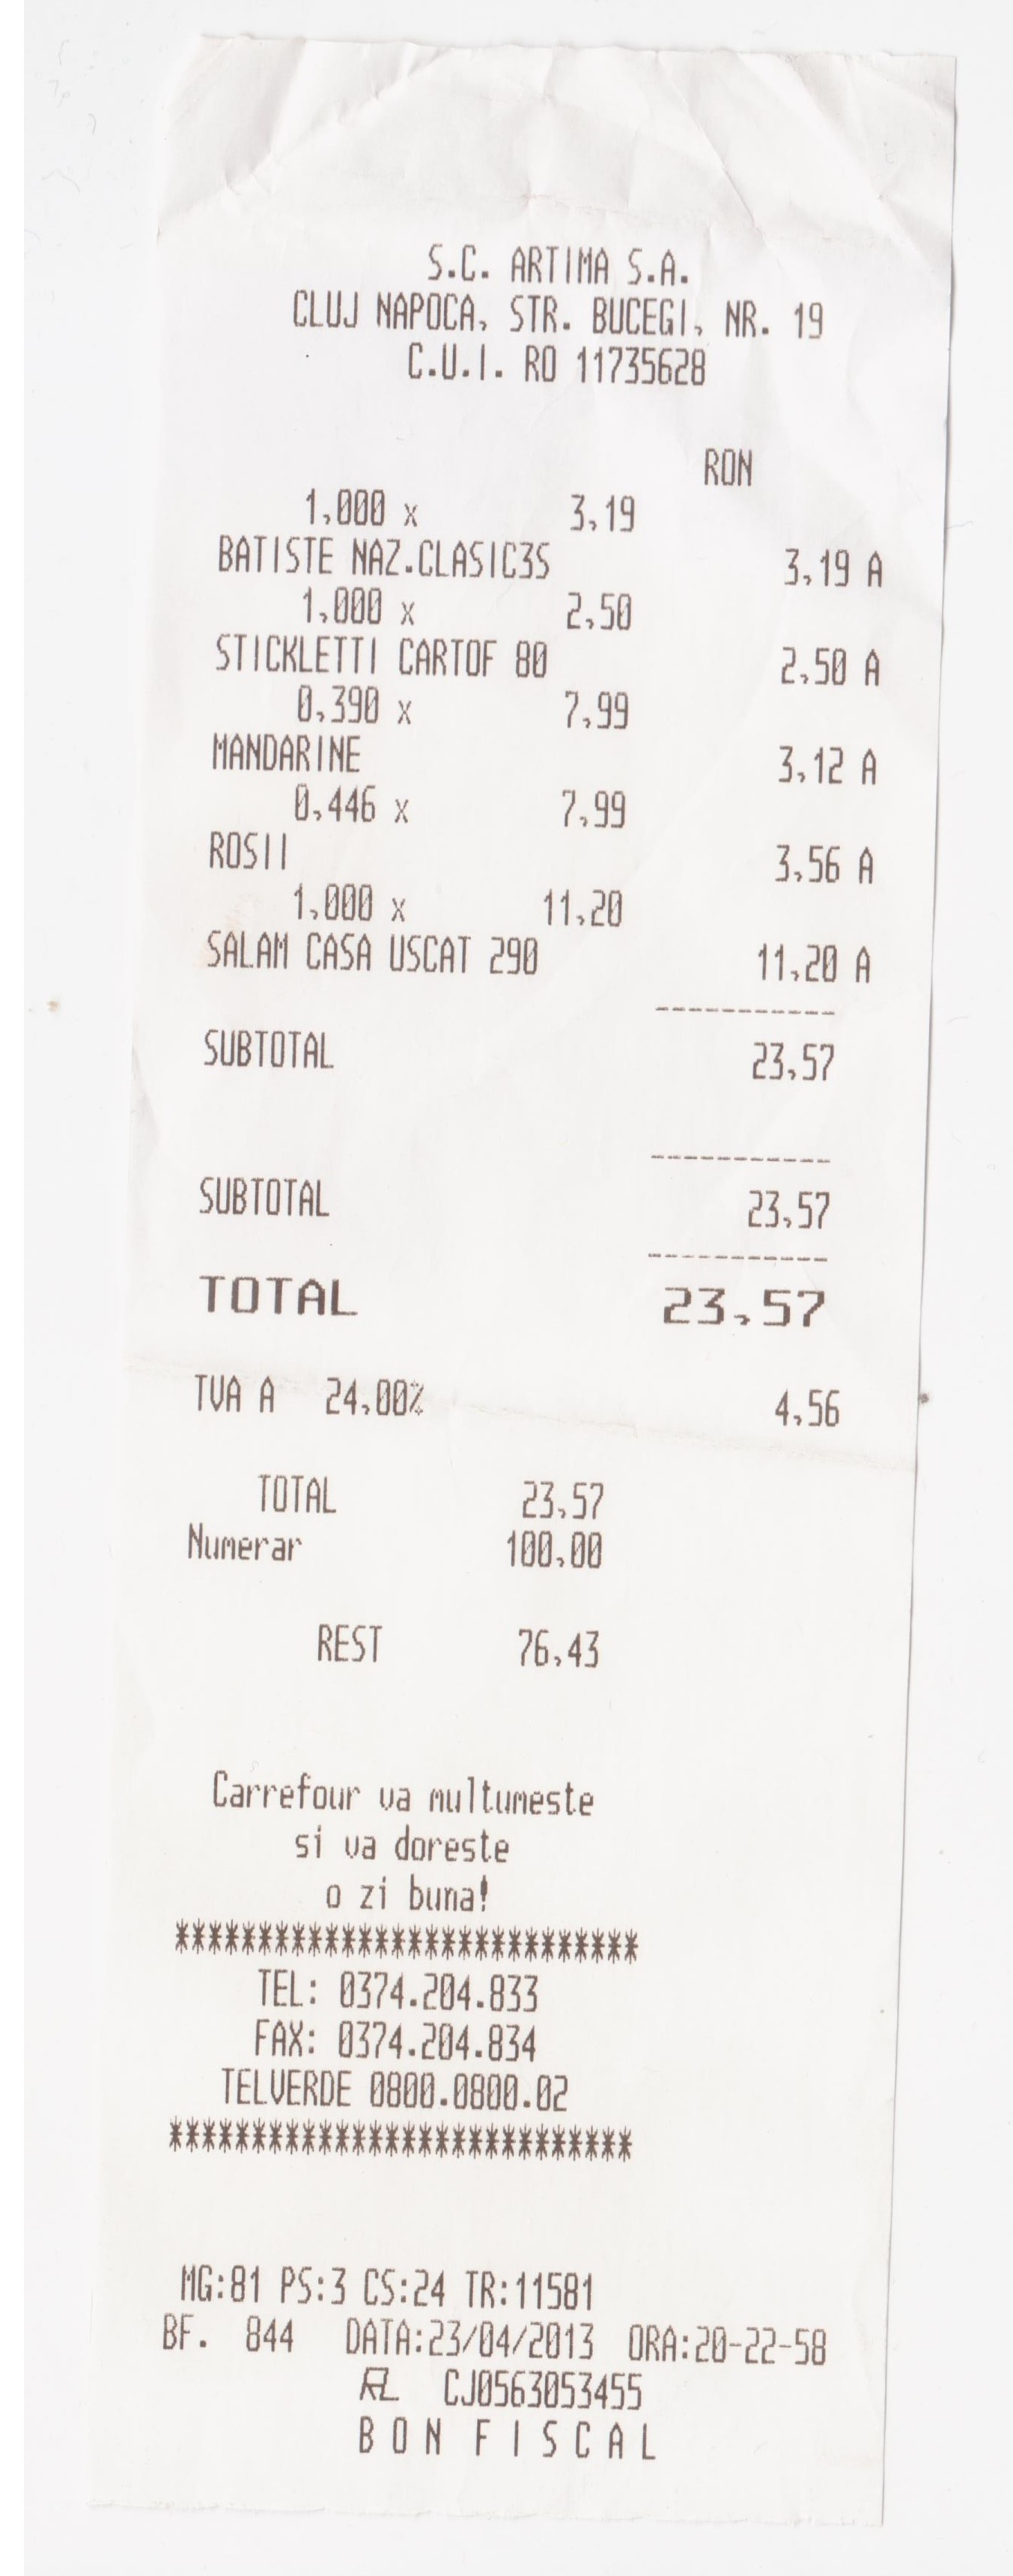
\includegraphics[width=.6\linewidth]{img/original.jpg}
  \caption{Original receipt image}
  \label{fig:orig_image}
\end{subfigure}
\begin{subfigure}{0.49\linewidth}
  \centering
  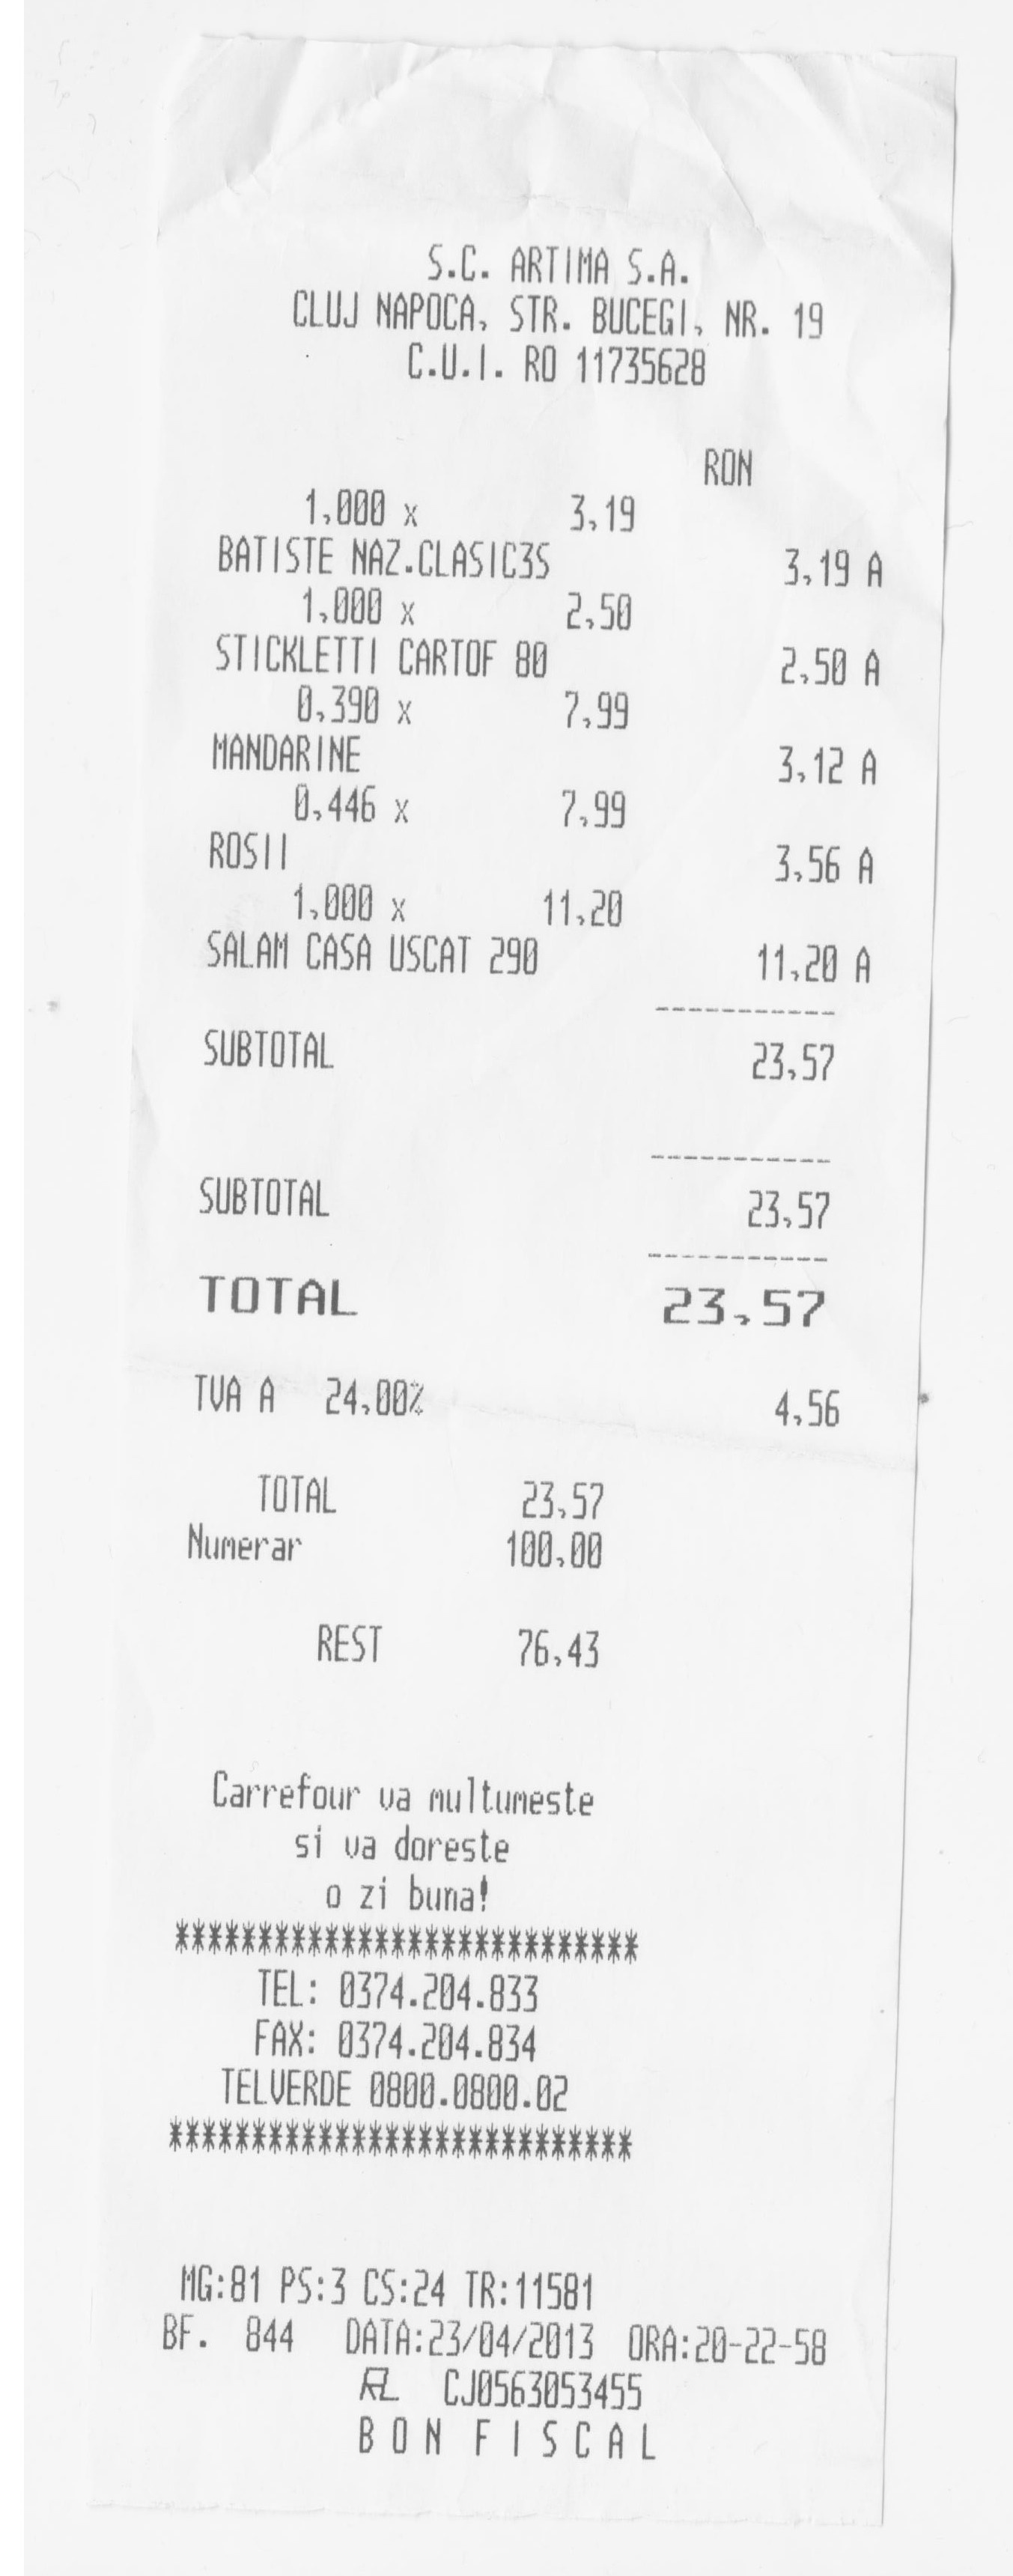
\includegraphics[width=.6\linewidth]{img/gray.jpg}
  \caption{Image converted to grayscale}
  \label{fig:gray_image}
\end{subfigure}
\begin{subfigure}{0.49\linewidth}
  \centering
  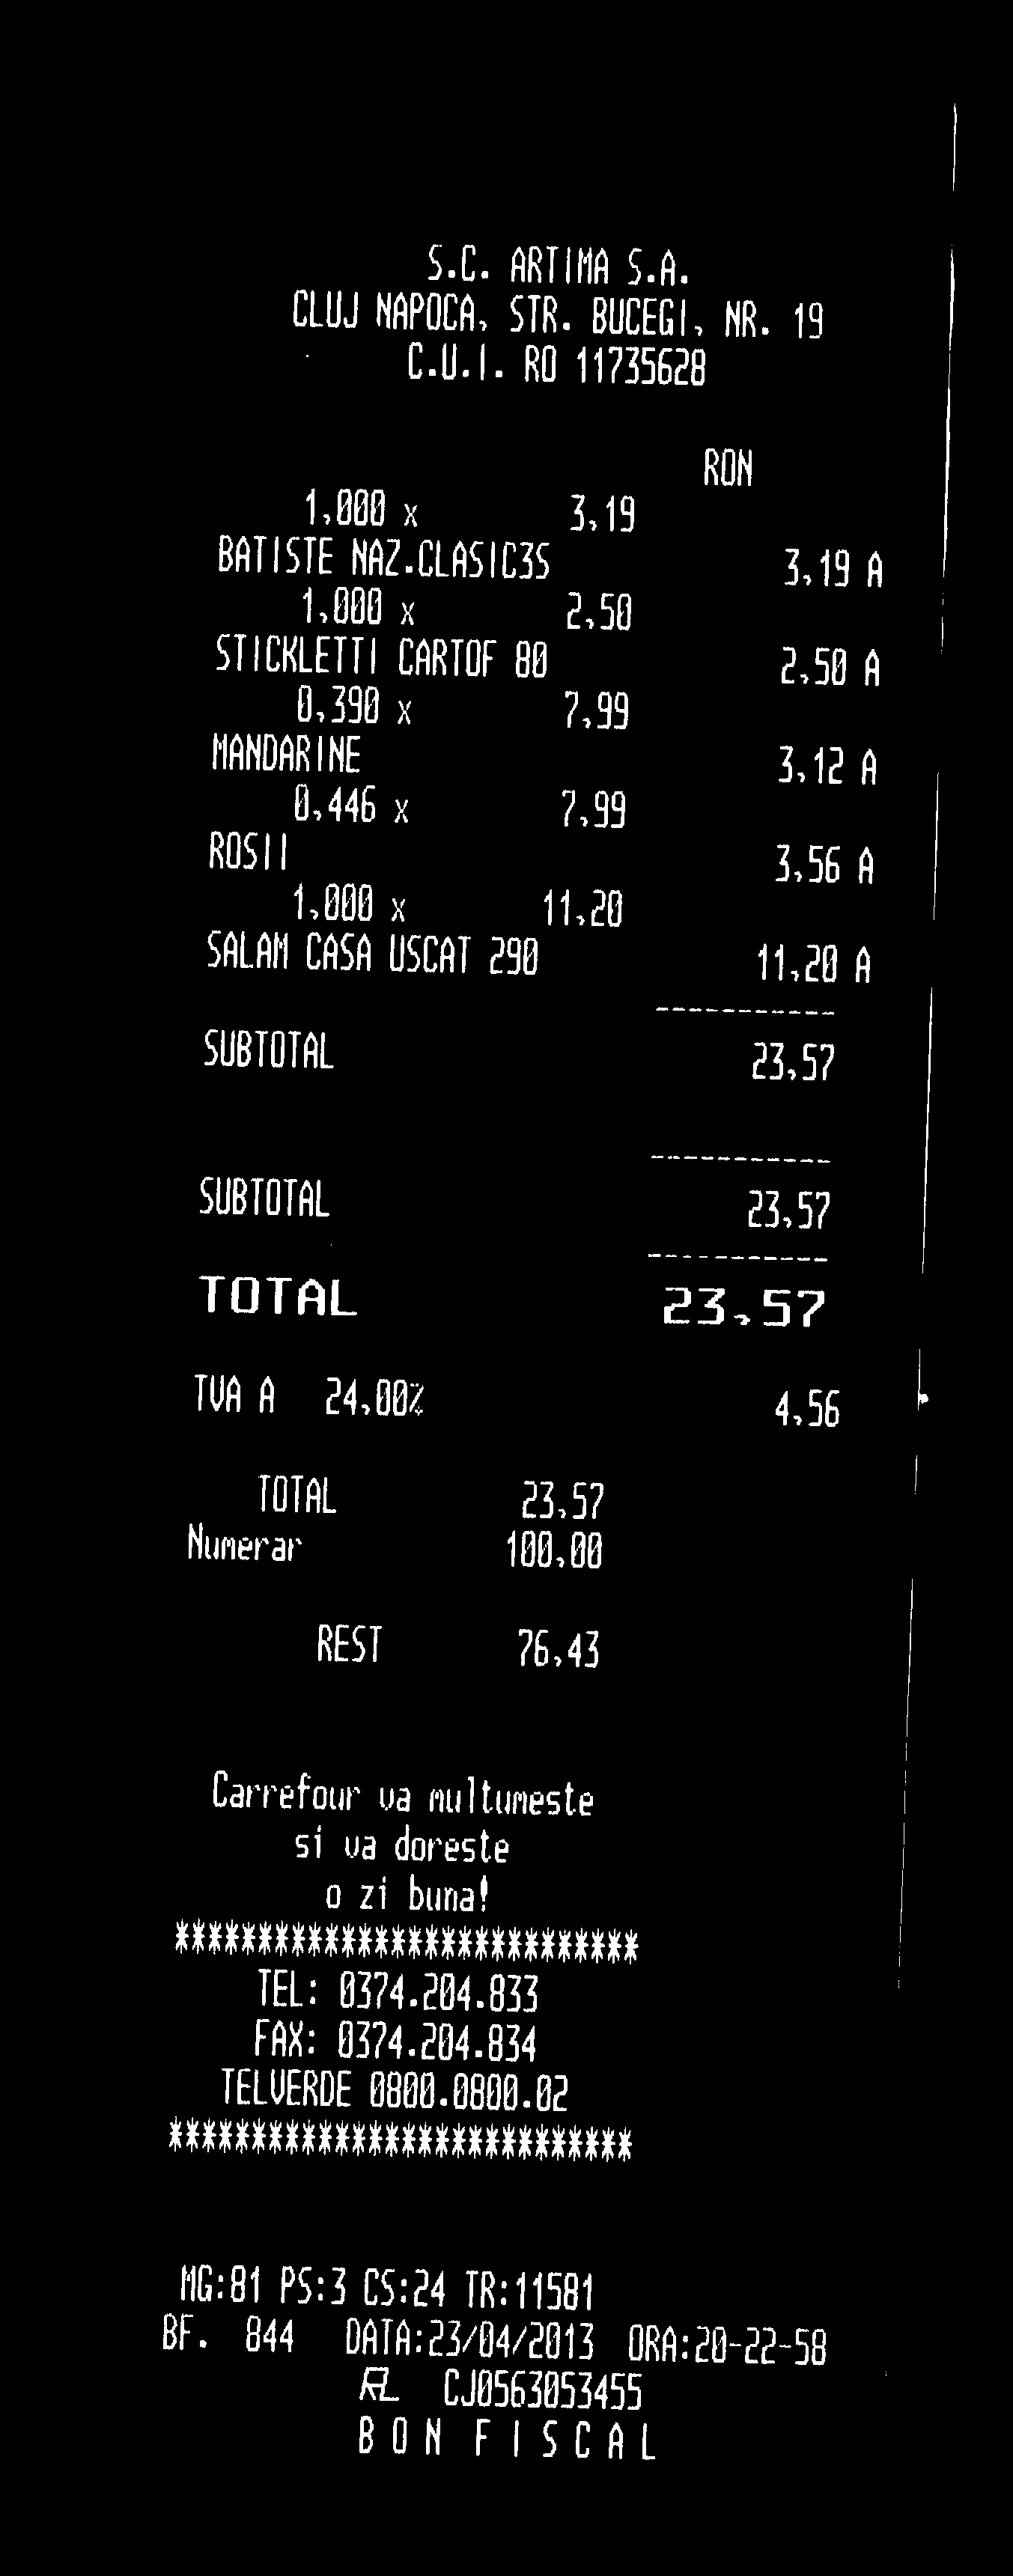
\includegraphics[width=.6\linewidth]{img/binarized.jpg}
  \caption{Binarized image}
  \label{fig:bin_image}
\end{subfigure}
\begin{subfigure}{0.49\linewidth}
  \centering
  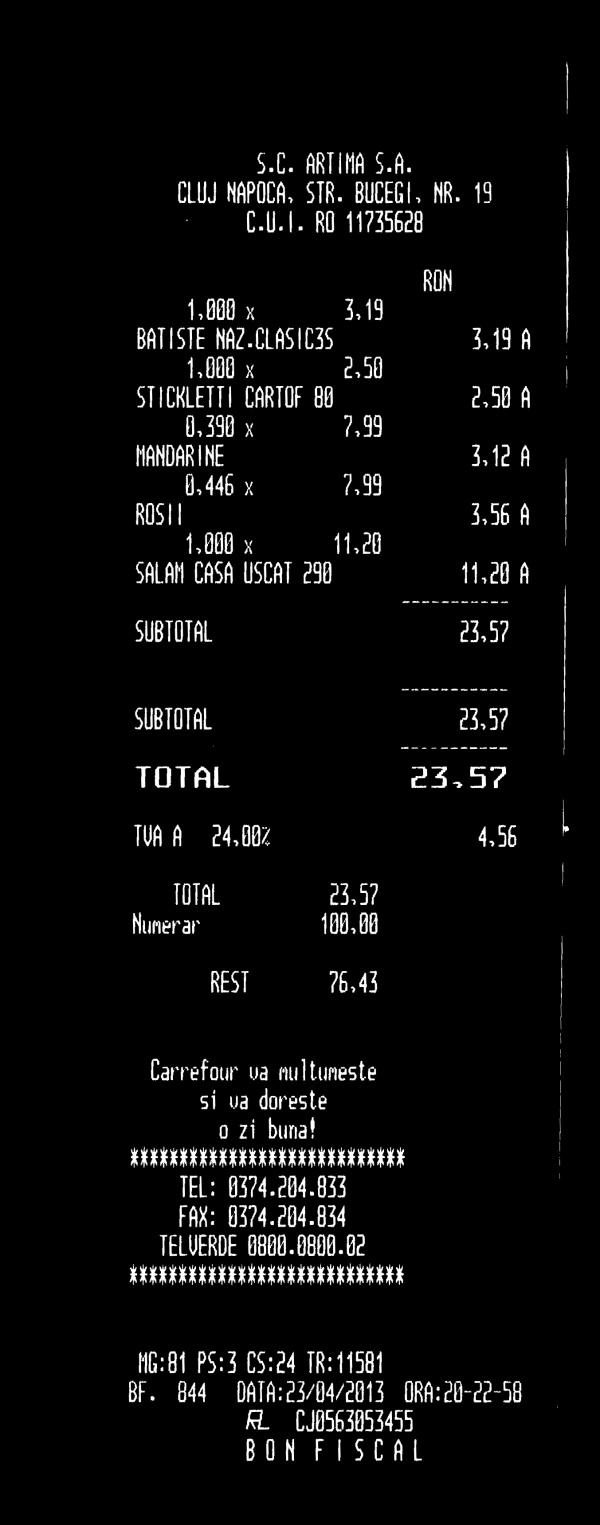
\includegraphics[width=.6\linewidth]{img/straight.jpg}
  \caption{Straigthened image}
  \label{fig:straight_image}
\end{subfigure}
\caption{\label{fig:receipts}
The first three steps of the preprocessing of figure \ref{fig:orig_image}. }
\end{figure}

\begin{figure}
\ContinuedFloat 
\centering
\begin{subfigure}{0.49\linewidth}
  \centering
  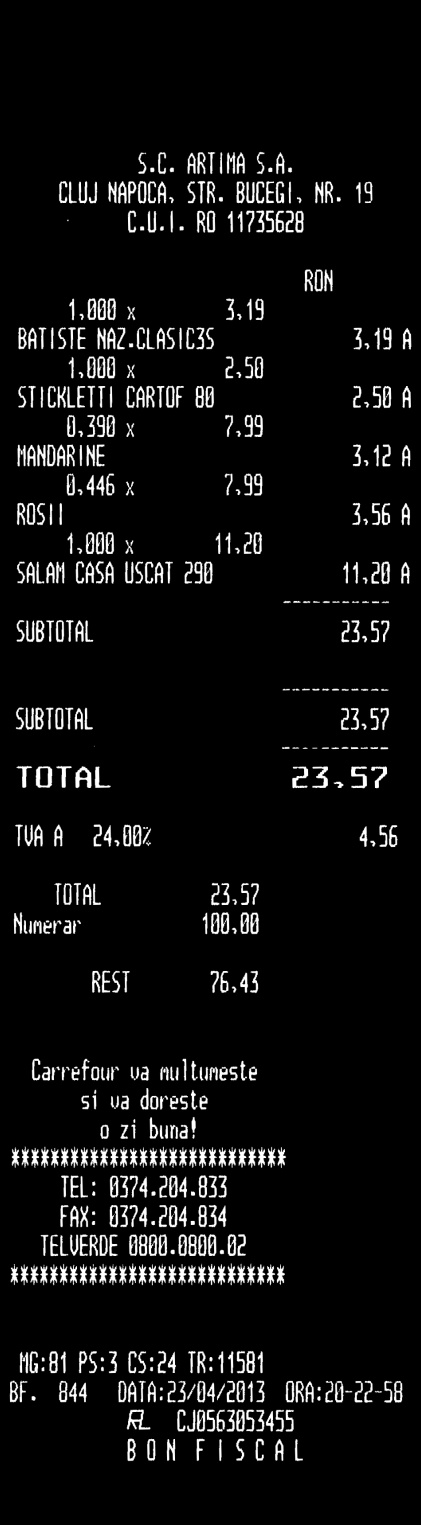
\includegraphics[width=.4\linewidth]{img/cleaned.jpg}
  \caption{Receipt after edge removal}
  \label{fig:edge_image}
\end{subfigure}
\begin{subfigure}{0.49\linewidth}
  \centering
i  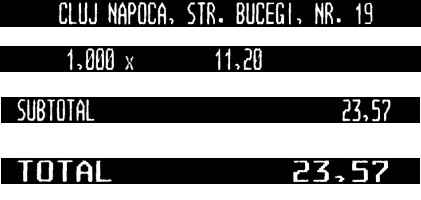
\includegraphics[width=\linewidth]{img/lines.jpg}
  \caption{Four lines extracted from the receipt}
  \label{fig:line_samples}
\end{subfigure}
\caption{\label{fig:receipts2}
The last step of the preprocessing of figure \ref{fig:orig_image} and some of the resulting lines. }
\end{figure}


\begin{figure}
\centering
\begin{subfigure}{\linewidth}
  \centering
  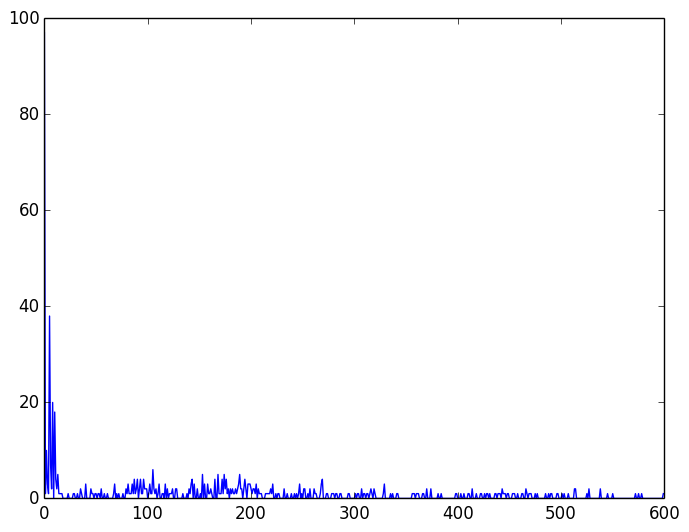
\includegraphics[width=\linewidth]{img/hist.png}
  \caption{Histogram of the number of pixels on each line}
  \label{fig:hist_plot}
\end{subfigure}
\begin{subfigure}{\linewidth}
  \centering
  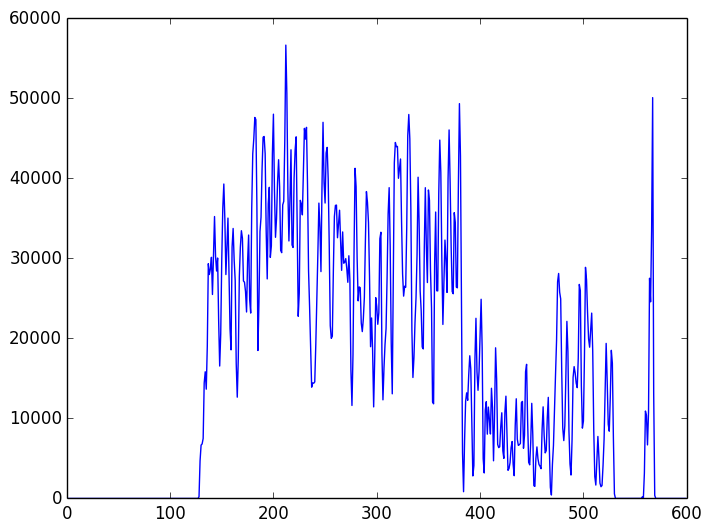
\includegraphics[width=\linewidth]{img/edges.png}
  \caption{Plot of the number of pixels on each column}
  \label{fig:edge_plot}
\end{subfigure}
\caption{\label{fig:plots}
The graphs with the values used to preprocess the receipt in Figure \ref{fig:orig_image}. }
\end{figure}

\begin{figure}
\ContinuedFloat
\centering
\begin{subfigure}{\linewidth}
  \centering
  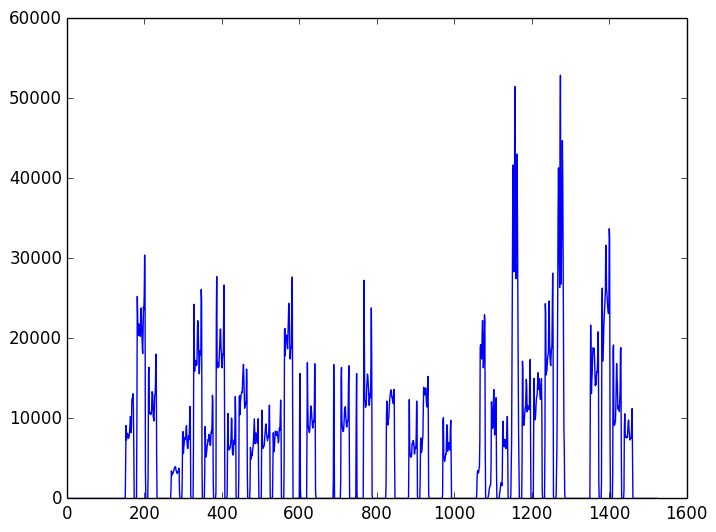
\includegraphics[width=\linewidth]{img/lines.png}
  \caption{Plot of the number of pixels on each line}
  \label{fig:line_plot}
\end{subfigure}
\caption{\label{fig:plots2} }
\end{figure}

\subsection{Extracting data from text}
After the text is recognized in images, it must be processed and brought to a usable form. There are 6 relevant pieces of information that can be extracted from a receipt: the name of the shop which emitted the receipt, the address of that shop, the Unique Identifying Code (CUI) given to the company by the government, the items that were bought, the date the sale was made, and the total sum of money paid. 

The approach used in this thesis to extract this information is a simple rule based based system, that looks at each line and checks if it matches some conditions, such as if it matches a regular expression, or the if the count of digits, letters and other characters on the line is in certain ranges, to try to classify each line in one of those categories. 

The name of the shop is identified by searching the line for the following regular expression: 

\begin{lstlisting}
'S\.?C\.?(.+?)(S.?R.?L.?)|(S[:.,]?A[:.,]?)'
\end{lstlisting}

This expression search for anything that starts with \textbf{S.C.} and ends with either a \textbf{S.R.L} or \textbf{S.A.}. Because the dots are small and they are likely to be misclassified or not recognized, they are made optional in the regular expression. Another condition that a line must satisfy is to be in the first 5 lines of the receipt. This is done to prevent detecting any oddly named items that might match this pattern. The only problem with this regular expression is that some shops belong to a different class of entities, such as Kaufland, which is a ``Societate în comandită''.

The unique identifier of the shop can come in multiple forms: it always contains at least 4 digits, sometimes is prefixed by \textbf{C.U.I}, \textbf{C.F.} or \textbf{C.I.F.}, and it must be in the first 6 lines of the receipt. Also, any line containing 8 consecutive digits is considered to be the unique identifier. The regular expression for this is given by:

\begin{lstlisting}
'(C[^\w]?U[^\w]?I[^\w]?)|(C[^\w]?F[^\w]?)|
 (C[^\w]?I[^\w]?F[^\w]?)|
 (COD FISCAL).+? (\d){4,}'
\end{lstlisting}

The address is locating by looking for one of two patterns. If the line is among the first 3 lines in the receipt and it contains the letters \textbf{NR} followed by digits, it is assumed to be an address. To other condition is if it is in the first 7 lines and it starts with either \textbf{STR}, \textbf{CALEA} or \textbf{B-DUL}. These regular expressions are the following:

\begin{lstlisting}
'(STR)|(CALEA)|(B-DUL).(.+?)'
'(NR).(\d+)'
\end{lstlisting}

If the substring \textbf{TVA} is found, the line is marked as a line containing the value added tax. This is not used anywhere else, but it helps reduce false classifications, because the item class is usually similar in structure. 

Totals are identified very simply, by looking for the substring \textbf{TOTAL} or \textbf{SUBTOTAL}.

Dates are identified by looking for a pattern that consists of two to four digits repeated three times, with either periods, commas or slashes between them. Optionally, it can be prefixed with \textbf{DATA}.

\begin{lstlisting}
'DATA?.+?\d{2,4}[.\\-]\d{2,4}[.\\-]\d{2,4}'
'\d{2}[./\\-]\d{2}[./\\-]\d{2,4}'
\end{lstlisting}

Items must occur before the line containing the \textbf{TOTAL}. Items sometimes have the name of the item and its price on the same line, but sometimes they are on two lines. The price part must have at least one character (usually for the currency), the ratio of digits to letters must be greater than one, it must be at least the third line in the receipt, but not in the last seven lines and the line most not contain \textbf{TEL} or \textbf{FAX}. The part with the item name must be at least the fourth line in a receipt, but before the last eight lines, it must have at least five letters and punctuation characters, and it must not contain any of the following \textbf{TEL}, \textbf{FAX}, \textbf{SUBTOTAL}, \textbf{NUMERAR}, \textbf{BRUT}, \textbf{NET} or any of the day names. 

Any other lines are classified as unknown and are not taken into consideration in the subsequent steps.   

\subsection{Data Set and Processing}
The data set was obtained from 20 receipts that were manually annotated with the position of each character in them. In total there are 7045 characters. There are 74 different characters, including digits, uppercase and lowercase letters and punctuation. 

The bounding boxes of the characters were extracted from the images. The resulting patches were normalized to have a size of 30x30 pixels and were converted to grayscale. The small images that resulted after this processing were used as the data set for the character recognition problem.

For the character segmentation problem, positive and negative patches were extracted from the images, each containing 40 columns of pixels. The positive example were obtained by taking the leftmost and rightmost columns of the bounding boxes of characters, together with 19 previous columns and 20 columns that followed. The negative examples were obtained by sampling randomly from the middle of a character and taking 19 columns from before and 20 from after.

For the character recognition problem, the labels corresponding to each character were converted to a vector of 74 dimensions, with each dimension corresponding to one possible character value. The value of the dimension corresponding to the character of a data point was set to 1, while all the others were set to 0. 

For the character segmentation problem, the labels were binary: 1 if a certain data point was were a segmentation should occur, 0 otherwise. 

For the neural network models the data set was augmented by moving each letter shape in the four possible directions by one pixel. This resulted in a five-fold increase in the number of data points available. This augmentation was not used in the case of the SVM because SVM training time is quadratic in the number of samples, and thus training time became unfeasible. 

\subsection{Training and Testing}
The data set was shuffled and then split into two parts, one for training and one for testing. The splitting was done in a random way, because the data points are independent and order does not matter. The training set contained 80\% of the data and the test set contained the remaining 20\%. 

All experiments were run multiple types, with the dataset being shuffled each time. In the case of the Random Forests, the multiple runs of the experiments are necessary because the splitting points for the trees and the dataset splits are chosen randomly across runs. In the case of the neural networks, the initialization of the weights between neurons was random. 
\subsection{Experimental evaluation}
\label{sec:recog}
In this section we describe the experiments that we have done, starting with the data gathering process, the training of the models and the results of their evaluation.

For both tasks, the parameters for the algorithms were selected using cross-validation. In the case of the SVM, the search space was on logarithmic scale from $10^{-2}$ to $10^4$ for the regularization parameter. In the case of the random forest, the number of trees used ranged from 150 to 250, in steps of 50, and the number of features to be sampled at each point varied from using the square root, the base 2 logarithm, 10\% or 30\% of the total number of features.

The neural networks were used in 4 configurations: 

\begin{description}


\item[Stacked Autoencoders (SAU)] - a two layered neural network pretrained with denoising autoencoders. Both layers had 500 neurons and their activation functions were hyperbolic tangent.  The input was randomly set to 0 with probability 0.2 for the first layer, and 0.3 for the second layer,
\item[MLP2] - a two layered neural network with ReLU units. The first layer had 1000 units, the second one had 800 units. Weight decay was applied to all layers,
\item[MLP3] - a three layered neural network with ReLU units, with 500, 400, 500 neurons per layer,
\item[MLP4] - a four layered neural network with ReLU units, in the configuration of 800, 1000, 800, 600 neurons per layer;
\end{description}

In all cases the learning rate was set to 0.8, the stochastic gradient descent algorithm was run for 100 iterations and there was an momentum of 0.5.

Table \ref{table:recog_values} contains the average, maximum and minimum values obtained as a baseline using an SVM for the accuracy of the character recognition problem.

\begin{table}[h]
\caption{The baseline for the accuracy of the character recognition experiment, using an SVM}
\label{table:recog_values}
\begin{tabular}{lrrrrr}
\toprule
Kernel type & Regularization & Min     & Max     & Mean    & Std. dev. \\ 
\midrule
RBF & 0.01 & 0.09141 & 0.09207 & 0.09165 & 0.00030 \\ 
Linear & 0.01 & 0.71585 & 0.71768 & 0.71672 & 0.00075 \\ 
RBF & 1 & 0.59146 & 0.60671 & 0.60130 & 0.00697 \\ 
Linear & 1 & 0.90372 & 0.90610 & 0.90490 & 0.00097 \\ 
RBF & 100 & 0.90854 & 0.91159 & 0.91018 & 0.00126 \\ 
Linear & 100 & 0.89695 & 0.90006 & 0.89860 & 0.00128 \\ 
RBF & 1000 & 0.90183 & 0.91341 & 0.90795 & 0.00475 \\ 
Linear & 1000 & 0.89207 & 0.89762 & 0.89453 & 0.00231 \\ 
RBF & 10000 & 0.90671 & 0.91220 & 0.90957 & 0.00225 \\ 
Linear & 10000 & 0.89146 & 0.89762 & 0.89494 & 0.00258 \\ 
\bottomrule
\end{tabular}
\end{table}

In this case, using RBF kernel SVM resulted in a $ 91.018\% \pm 0.126 $ accuracy in the best case, using a value of 100 for the regularization rate, while using a linear kernel yielded $ 90.490\% \pm 0.097 $ as its best result, for the value of 1 for the regularization rate. A RBF kernel gives a slightly better results.

The results obtained from the neural networks can be seen in table \ref{table:nn_table}, with the minimum, maximum, mean and standard deviation shown for all four configurations, the experiments being run 5 times. 

\begin{table}[h]
\caption{The accuracy for the character recognition experiment using the neural network configurations}
\label{table:nn_table}
\begin{tabular}{lrrrr}
\toprule
Neural network & Min     & Max     & Mean    & Std. dev. \\ 
\midrule
SAU & 0.95122 & 0.96113 & 0.95625 & 0.00387 \\ 
MLP2 & 0.95808 & 0.98780 & 0.97988 & 0.01244 \\ 
MLP3 & 0.94512 & 0.98857 & 0.97576 & 0.01768 \\ 
MLP4 & 0.98171 & 0.98780 & 0.98506 & 0.00256 \\ 
\bottomrule
\end{tabular}
\end{table}

Figure \ref{fig:conf_matrix} contains the confusion matrix for the best experiment on the character recognition problem.


\begin{figure}[h!]
\begin{center}
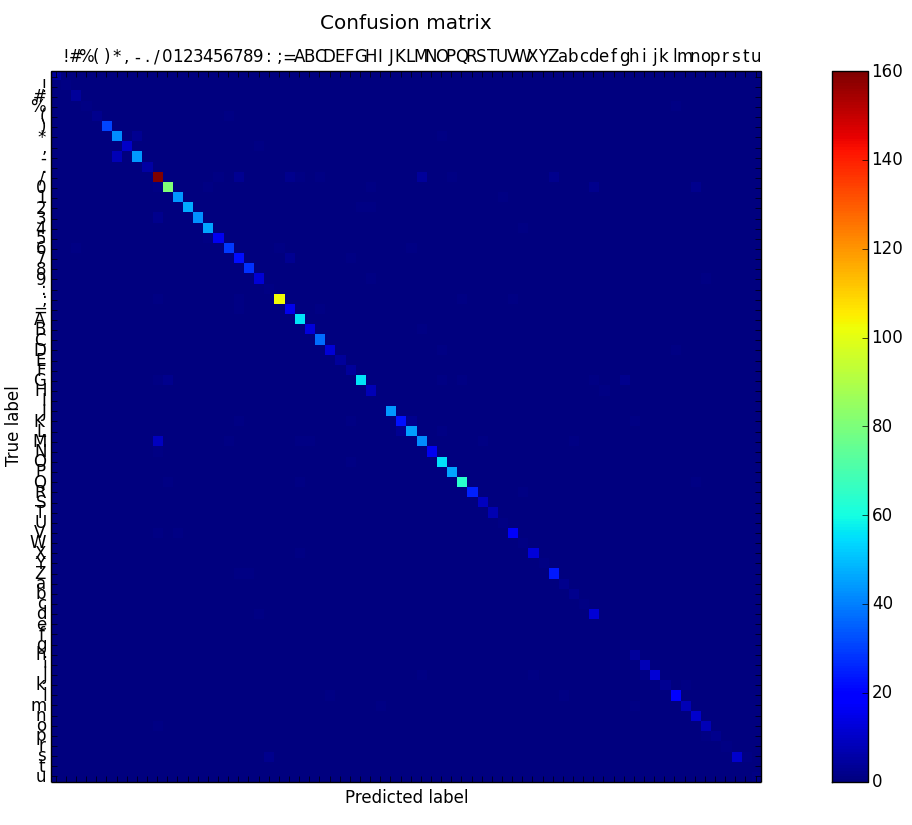
\includegraphics[width=0.8\linewidth]{img/rec_cm.png}
\caption{\label{fig:conf_matrix}
Confusion matrix for the best model for the character recognition problem}
\end{center}
\end{figure}

Table \ref{table:seg_values} contains the average, maximum and minimum values obtained for the F1 measure\cite{fawcett2006introduction} of the character segmentation problem. The F1 measure is used instead of the accuracy because the two classes are imbalanced: there are 11475 data points which indicate a segmentation point, while there are 19402 points which are not segmentation points, almost twice as many. 

\begin{table}[h]
\caption{The F1 score for the character segmentation experiment}
\label{table:seg_values}
\begin{tabular}{llllll}
\toprule
Nr. trees & Nr. features & Min     & Max     & Mean    & Std. dev. \\ 
\midrule
150 & 20 & 0.87318 & 0.88326 & 0.87735 & 0.00363 \\ 
200 & 20 & 0.86975 & 0.88312 & 0.87657 & 0.00490 \\ 
250 & 20 & 0.87258 & 0.88776 & 0.87773 & 0.00531 \\ 
150 & 8 & 0.86894 & 0.88376 & 0.87569 & 0.00517 \\ 
200 & 8 & 0.87227 & 0.88299 & 0.87675 & 0.00413 \\ 
250 & 8 & 0.87178 & 0.88470 & 0.87717 & 0.00426 \\ 
150 & 120 & 0.87262 & 0.88631 & 0.87816 & 0.00476 \\ 
200 & 120 & 0.87122 & 0.88387 & 0.87724 & 0.00418 \\ 
250 & 120 & 0.87367 & 0.88565 & 0.87885 & 0.00391 \\ 
150 & 40 & 0.87073 & 0.88671 & 0.87822 & 0.00552 \\ 
200 & 40 & 0.86980 & 0.88519 & 0.87845 & 0.00513 \\ 
250 & 40 & 0.87358 & 0.88671 & 0.87936 & 0.00445 \\ 
\bottomrule
\end{tabular}
\end{table}

The confusion matrix for the best experiment on the character segmentation problem is presented in table \ref{table:seg_conf}.

\begin{table}[h]
\caption{The confusion matrix for the character segmentation experiment}
\label{table:seg_conf}
\begin{tabular}{lll}
\hline
 & No split & Split \\ \hline
Predicted no split & 4556 & 363 \\ 
Predicted split & 255 & 2546 \\  \hline
\end{tabular}
\end{table}

In table \ref{table:line_identify} we can see the confusion matrix for the line classification problem, showing how many times each class of lines was correctly classified and how often was it mistaken for something else. 

\begin{table}[h]
\caption{The confusion matrix for the line identification problem}
\label{table:line_identify}
\begin{tabular}{lrrrrrrrrr}
\toprule
{} &  Address &  CUI &  Data &  Name &  Price &  Shop &  Total &  TVA &  Misc. \\
\midrule
Address &       62 &    0 &     0 &     3 &      0 &     0 &      0 &    0 &        0 \\
CUI     &        0 &   50 &     0 &     2 &      0 &     0 &      0 &    0 &        5 \\
Data    &        0 &    0 &    53 &     0 &      0 &     0 &      0 &    0 &        2 \\
Name    &        0 &    0 &     0 &   169 &      2 &     0 &      0 &    0 &       43 \\
Price   &        0 &    2 &     0 &     0 &    173 &     0 &      0 &    0 &        6 \\
Shop    &        0 &    0 &     0 &     0 &      0 &    55 &      0 &    0 &        0 \\
Total   &        0 &    0 &     0 &     0 &      0 &     0 &     79 &    0 &        0 \\
TVA     &        0 &    0 &     0 &     1 &      0 &     0 &      0 &   68 &        0 \\
Misc.   &        5 &    5 &     3 &     8 &      8 &     3 &      2 &    0 &      580 \\
\bottomrule
\end{tabular}
\end{table}

The evolution of the performance of the neural networks can be seen in Figure \ref{fig:nn_iteration}. The first 20 iterations are cut off so that the improvements from the end can be seen better. 

\begin{figure}[h!]
\begin{center}
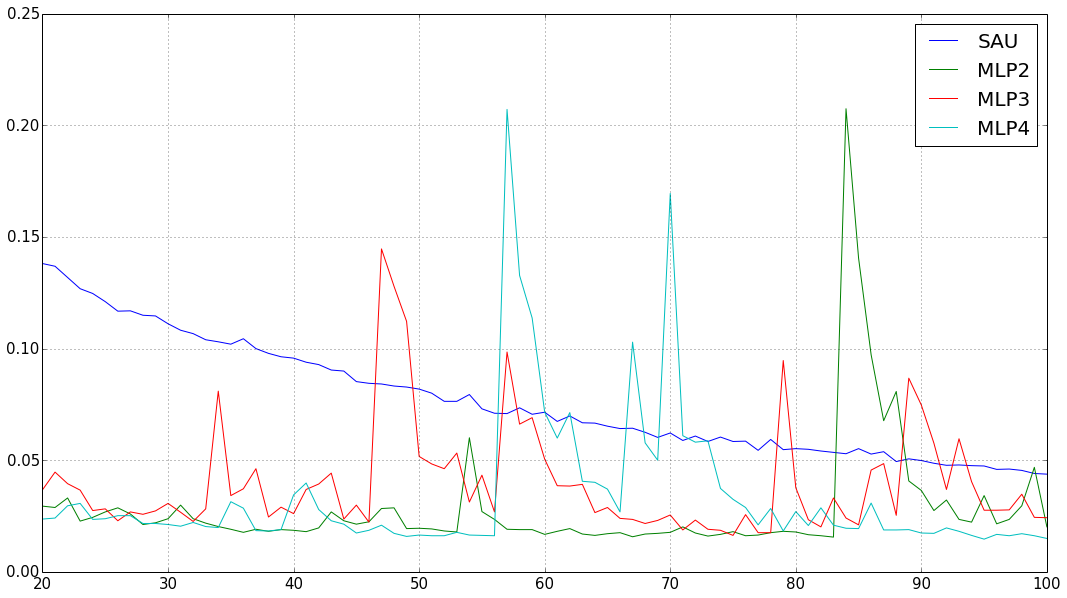
\includegraphics[width=\linewidth]{img/nn_iteration.png}
\caption{\label{fig:nn_iteration}
Evolution of the number of misclassifications made by the neural networks  starting from the 20th iteration until the 100th one}
\end{center}
\end{figure}
\section{Development}

\subsection{Used frameworks and libraries}
ReceiptBudget is a web application written in Python, using the Django framework  \cite{django}. Django is a high-level framework for doing rapid Web development in Python. It provides an out-of-the-box administration interface, an object-relational mapper that allows models to be written in Python, without any SQL code, a URL routing framework and a powerful templating system.

The maps of the dashboard were developed using the Google Maps API v3 \cite{gmapsjs}, which provides the mapping service for the heatmaps. The d3.js libray \cite{bostock2011d3} is the backbone of the dashboard. It provides a declarative way to view data in all kinds of visual ways and to make them interactive. The dc.js is a visualization framework built on top of d3.js which provides several standard graphical views, such as bar charts, pies, line charts. To provide a way to filter and drill down the data the crossfilter Javascript is used, which provides fast multidimensional filtering for coordinated views, allowing the user to select a subset of the data in one chart and updating the other charts to only include data from that subset. 

For the processing of the image the OpenCV libray is used, with its Python bindings. The scikit-learn library \cite{pedregosa2011scikit} is used for the random forest and SVM implementations, while the neural networks are used from the pylearn2 library \cite{goodfellow2013pylearn2}. 
\subsection{Requirements Analysis}
The application needs to support multiple users. New users can create an account by registering. After that they can import a CSV file that was exported from other finance management software. 

An authenticated user can then start inserting his expenses. He has three ways to do this. The first one is to take a picture of the receipt using a webcam. The second is to upload a photo containg a receipt from his harddrive. The last option is to enter the details of the receipt manually. 

In the dashboard, the user has three views where he can visualize his expenses. He can see a heat map of all his expenses. Another view is a dynamic heat map that shows the progression of his expenses day by day. The last view is the one which contains the interactive charts and graphs. Here the user can see detailed breakdowns of his expenses by day of week, shop, months and date range, hopefully noticing any negative spending patterns that can be cut down. 

If a users expenses for the past week are over the average weekly expenses, they will receive a visual warning, reminding them to be careful with what they spend their money on. This warning comes as a bright colored bar at the top of the screen, with the intensity of the color depending on how much the user stepped over the normal expense range. 
\subsection{Design}
The default administration provided by the Django framework is customized to make it fit together with the rest of the website, both from a UI perspective and from a security point of view. By default, the administration interface shows every existent object from the database. This is changed so that it shows only the expenses that belong to the current user. These changes are done by subclassing the default admin classes and registering the child classes instead of them. The corresponding UML diagram can be seen in Figure \ref{fig:admin_classes}.
\begin{figure}[h!]
\begin{center}
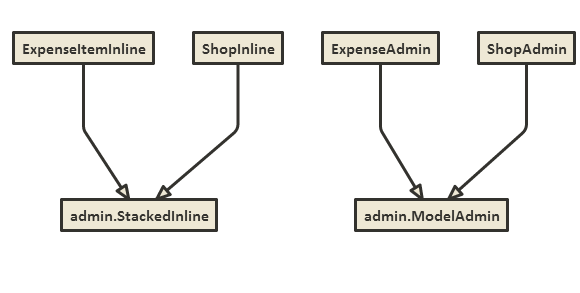
\includegraphics[width=\linewidth]{img/admin_classes.png}
\caption{\label{fig:admin_classes}
The classes used for the administration interface of the application}
\end{center}
\end{figure}

There are four entities that need to be stored in the database. One of them is a user entity, which is provided by the Django framework with everything it needs, including a profile, registration, password recovery and other security measures. 

The other entities are a \textbf{Shop}, where expenses can be made, an \textbf{Expense}, which has expense items, and \textbf{ExpenseItems}, which are the atomic elements of spending. 

Shops have a name, an address, a CUI and geographical coordinates. These are determined from the address via a geocoding service, such as the one offered by Google. The geographical coordinates are stored in the database, even though they are computable attributes because making the call to an external service is costly and because the number of calls that can be made per second is limited. Because of this, whenever a new shop is introduced, or when an existing shop is modified, a call is made to determine its location. This location is then used to plot on the heatmap.

Expenses have a date on which they were made and a user to whom they belong. They must have at least one Expense Item, but up to any number of them. They provide a property to calculate the total amount spent, by summing all the individual expenses. 

Expense items have a name and a price associated with them and represent the fundamental element where money is spent. They are individual items that can be bought. 

The UML diagram showing these classes can be seen in Figure \ref{fig:classes}.

\begin{figure}[h!]
\begin{center}
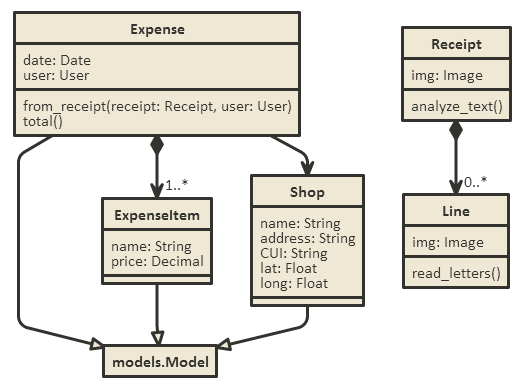
\includegraphics[width=\linewidth]{img/classes.png}
\caption{\label{fig:classes}
UML diagram of the classed used for the models and for the OCR engine}
\end{center}
\end{figure}

The OCR engine has two entities: receipts and lines. A receipt can have multiple lines. The receipt is responsible for cleaning up the input image, preprocessing it and finding the lines in it, which are then instantiated as separate objects which perform the actual process of character segmentation and recognition. After all the lines have finished recognizing, the receipt object can classify its lines and then it can return the properties of the receipt: date, shop, CUI, address, items, total. 

% \subsection{Implementation}
% mai trebuie asta?

\subsection{User Manual}
\label{sec:manual}

When a user comes to the ReceiptBudget website, he is presented with the main landing page, which can be seen in Figure \ref{fig:intro}. If he has an account, he can log in, if not he can create an account, using the form in Figure \ref{fig:register}, after which he is logged in automatically.

\begin{figure}[htdp]
\begin{center}
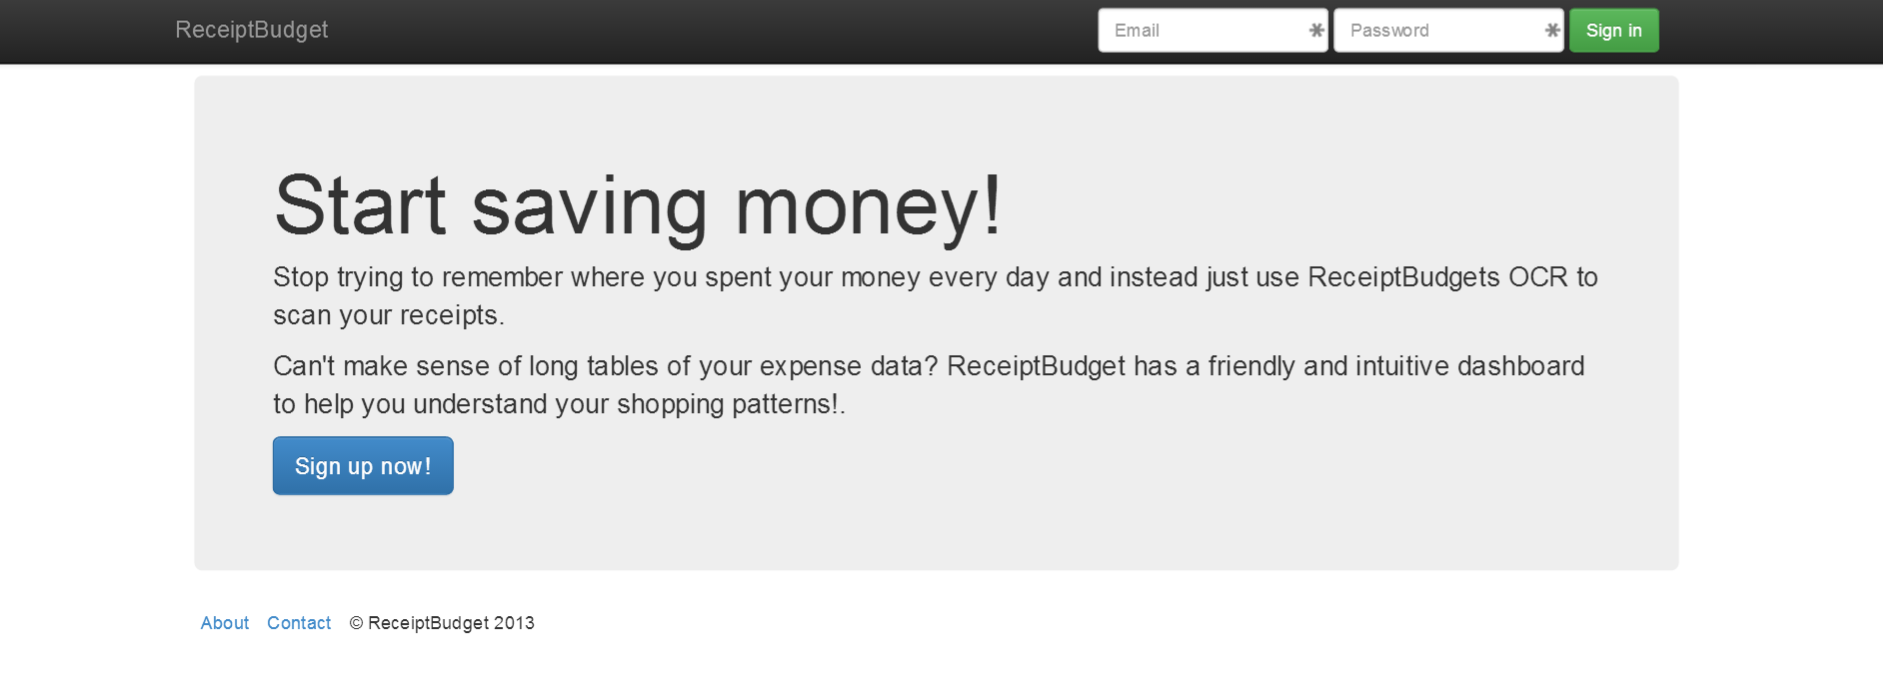
\includegraphics[width=\linewidth]{img/manual/intro.png}
\caption{\label{fig:intro}
The home page shown to a user who is not yet logged-in}
\end{center}
\end{figure}

\begin{figure}[htdp]
\begin{center}
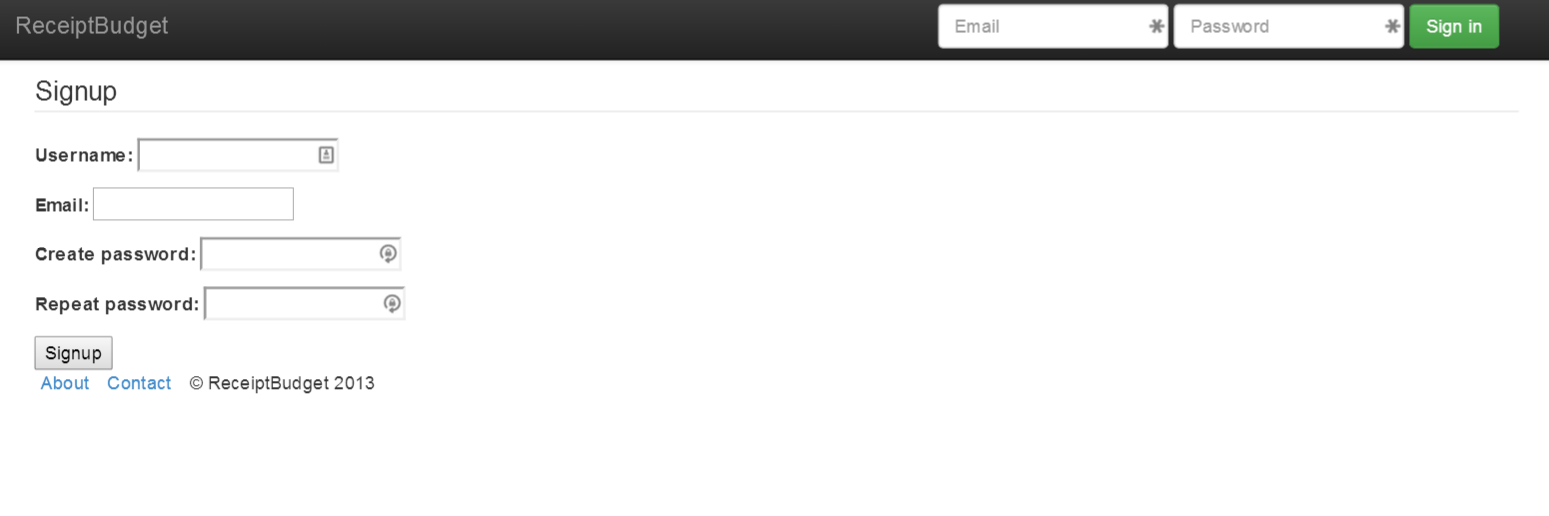
\includegraphics[width=\linewidth]{img/manual/register.png}
\caption{\label{fig:register}
The registration screen}
\end{center}
\end{figure}

After a user has logged in, he is presented with a list of his expenses, similar to the one in Figure \ref{fig:expense_list}. He can then choose to add a new expense, edit an existing one, view the dashboard or edit his user profile. 
\begin{figure}[htdp]
\begin{center}
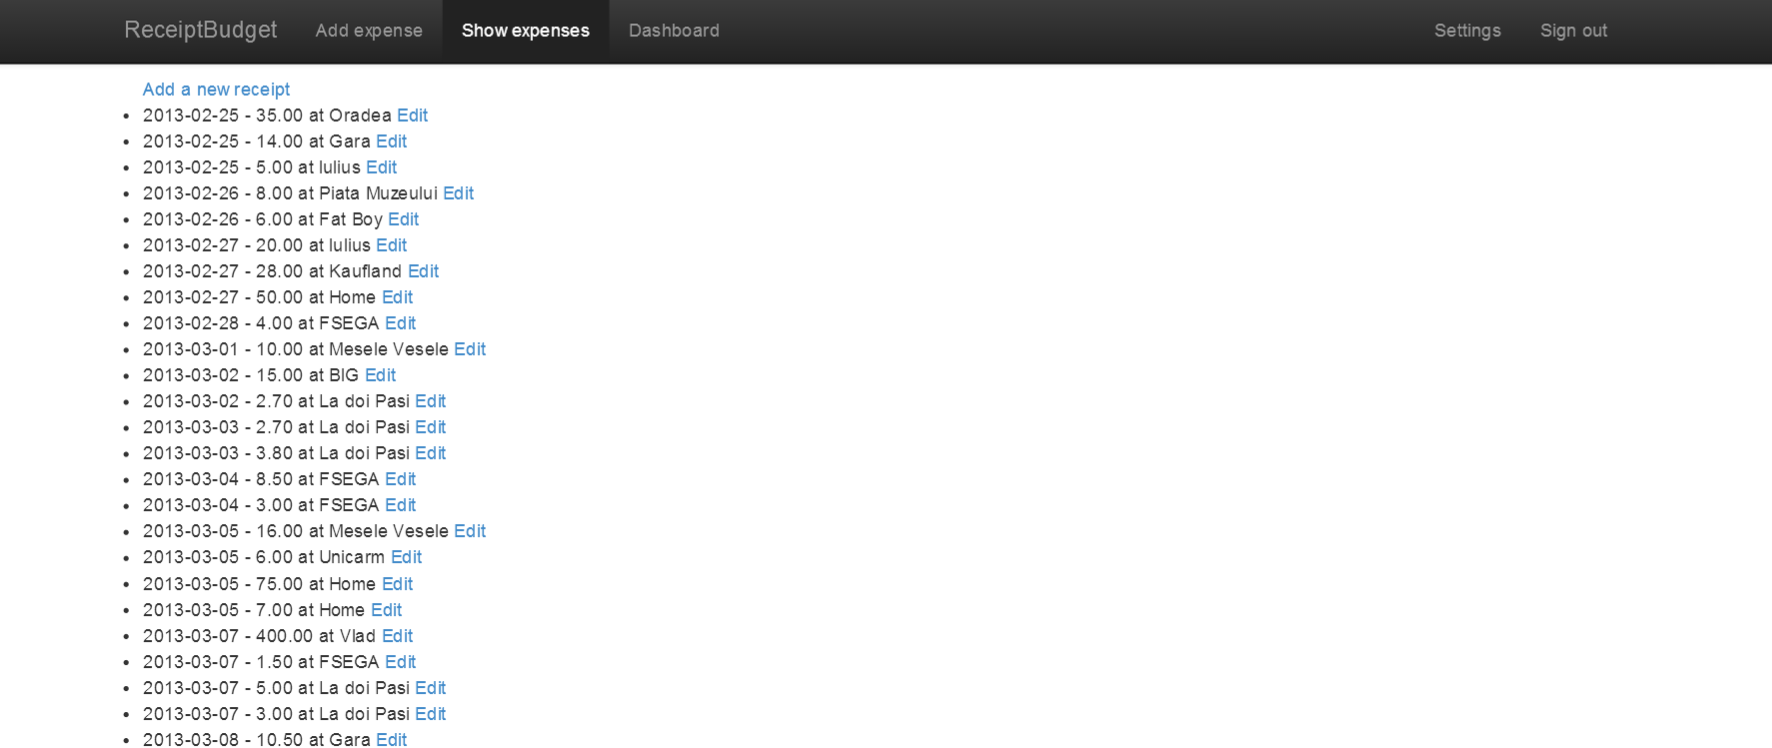
\includegraphics[width=\linewidth]{img/manual/expense_list.png}
\caption{\label{fig:expense_list}
The main page shown to a logged-in user}
\end{center}
\end{figure}

In their user profile (Figure \ref{fig:user_profile}) they can change personal information, such as name, picture and privacy settings (Figure \ref{fig:profile_edit}), their email address or their password.

\begin{figure}[htdp]
\begin{center}
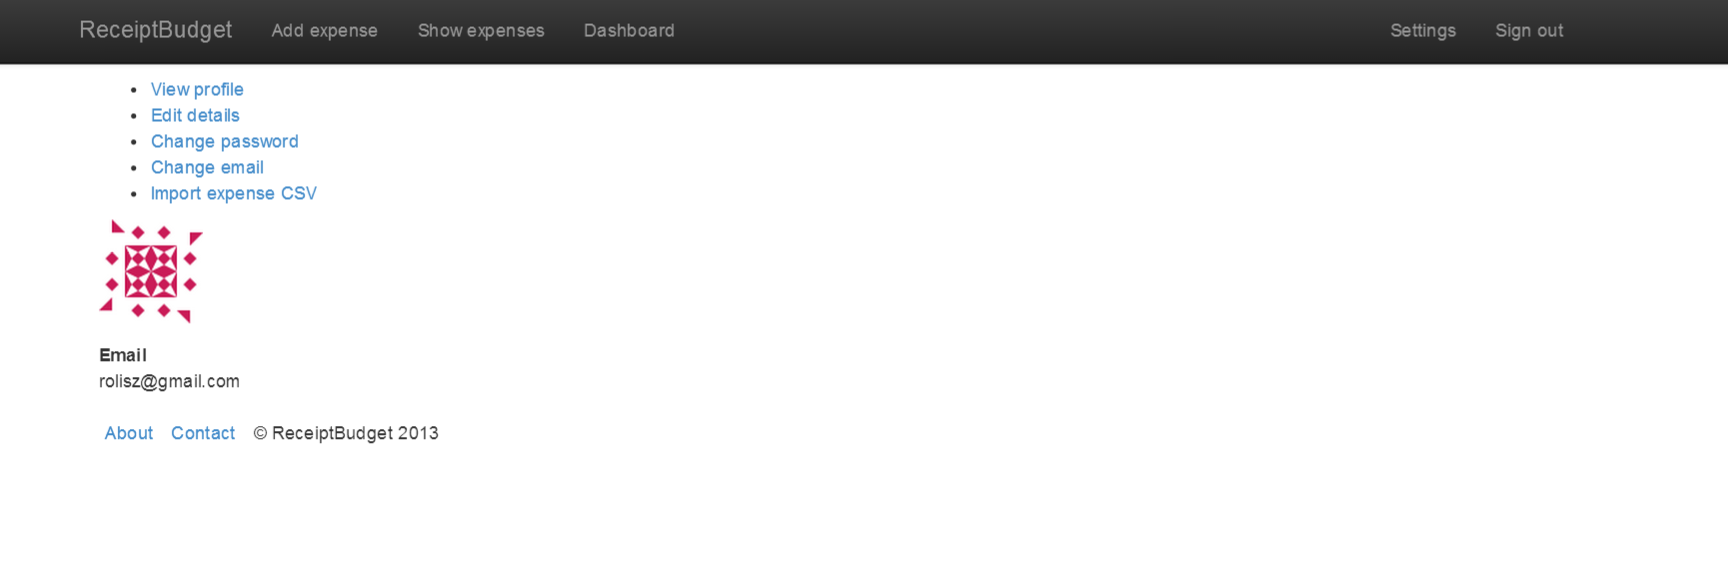
\includegraphics[width=\linewidth]{img/manual/user_profile.png}
\caption{\label{fig:user_profile}
The user profile screen}
\end{center}
\end{figure}

\begin{figure}[htdp]
\begin{center}
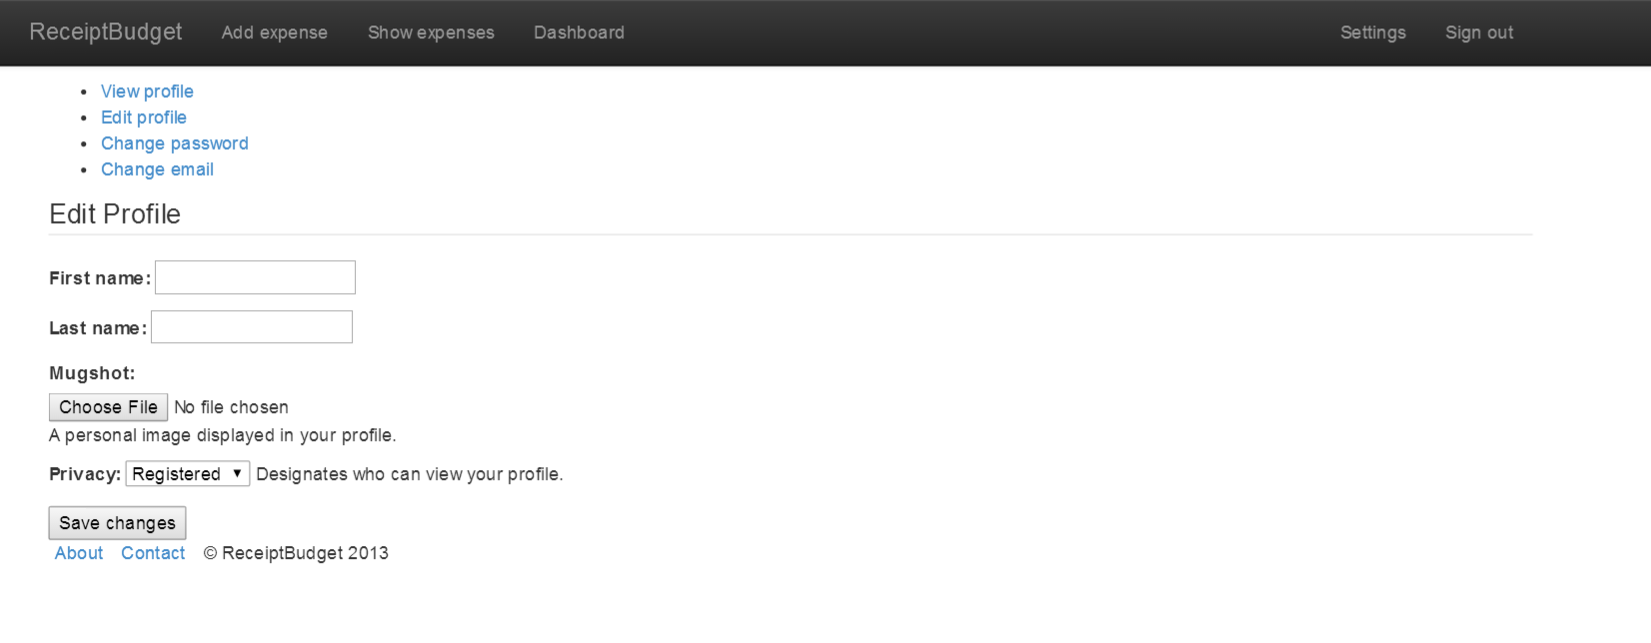
\includegraphics[width=\linewidth]{img/manual/profile_edit.png}
\caption{\label{fig:profile_edit}
The screen for editing the user's own profile}
\end{center}
\end{figure}

On their own personal settings page, the user can import previous expenses that were exported from another personal finance manager in a CSV format. The import tool will try to guess which column from the CSV file corresponds to the internal data structures used by ReceiptBudget and uses heuristics to determine which is the date, expense name, expense value and location where the expense was made. The user has the possibility to correct the guesses made by the application using the screen seen in Figure \ref{fig:csv_import}.

\begin{figure}[htdp]
\begin{center}
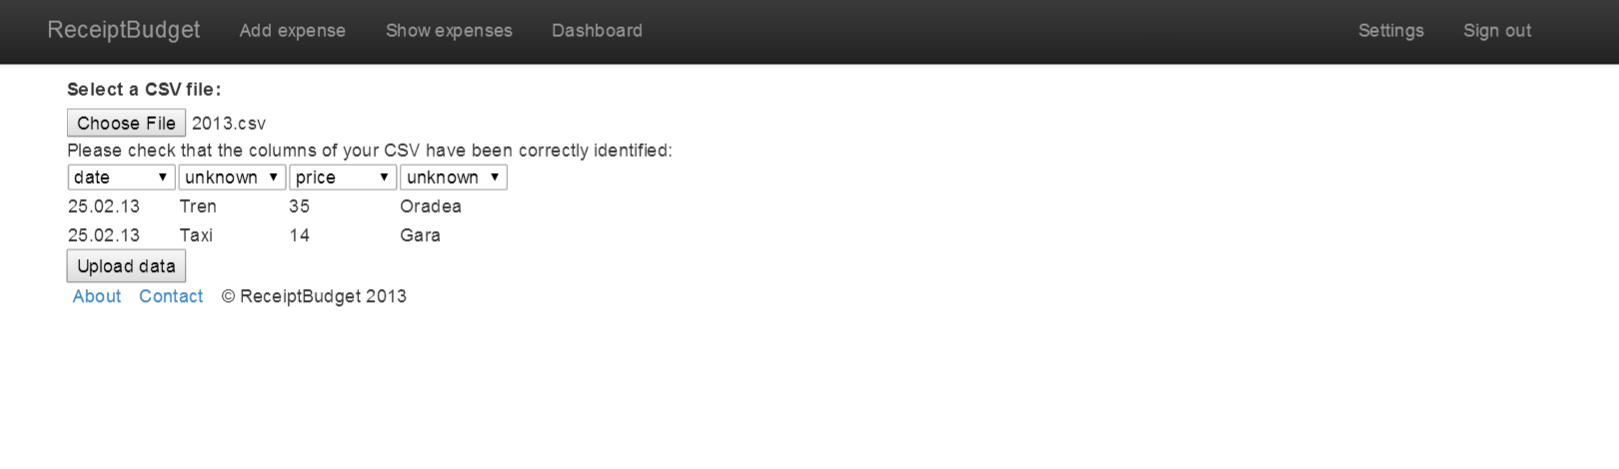
\includegraphics[width=\linewidth]{img/manual/csv_import.png}
\caption{\label{fig:csv_import}
Importing a CSV file containing financial data exported from other programs}
\end{center}
\end{figure}

If a user chooses to add an expense, he has three options. He can add a new expense manually, which is useful for cases where there is no receipt or it was lost, using the form from Figure \ref{fig:manual_add}. Another option would be to add a receipt from an image that is saved on the computer. The last option is to take an image of a receipt with a webcam. In this case the user has to align the receipt and after taking the picture he can select the bounding box for the receipt as seen in Figure \ref{fig:webcam}, and after that he can upload the image to the server. 

\begin{figure}[htdp]
\begin{center}
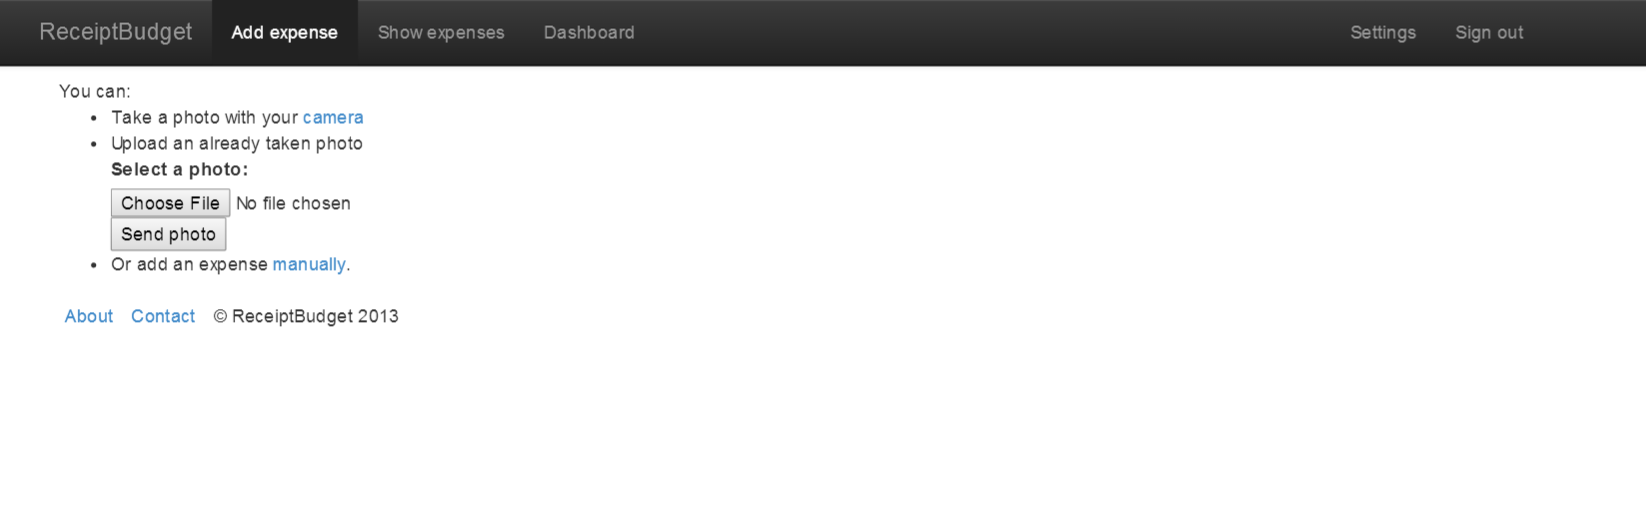
\includegraphics[width=\linewidth]{img/manual/add_expense.png}
\caption{\label{fig:add_expense}
Main screen showing the three options for adding expenses}
\end{center}
\end{figure}

\begin{figure}[htdp]
\begin{center}
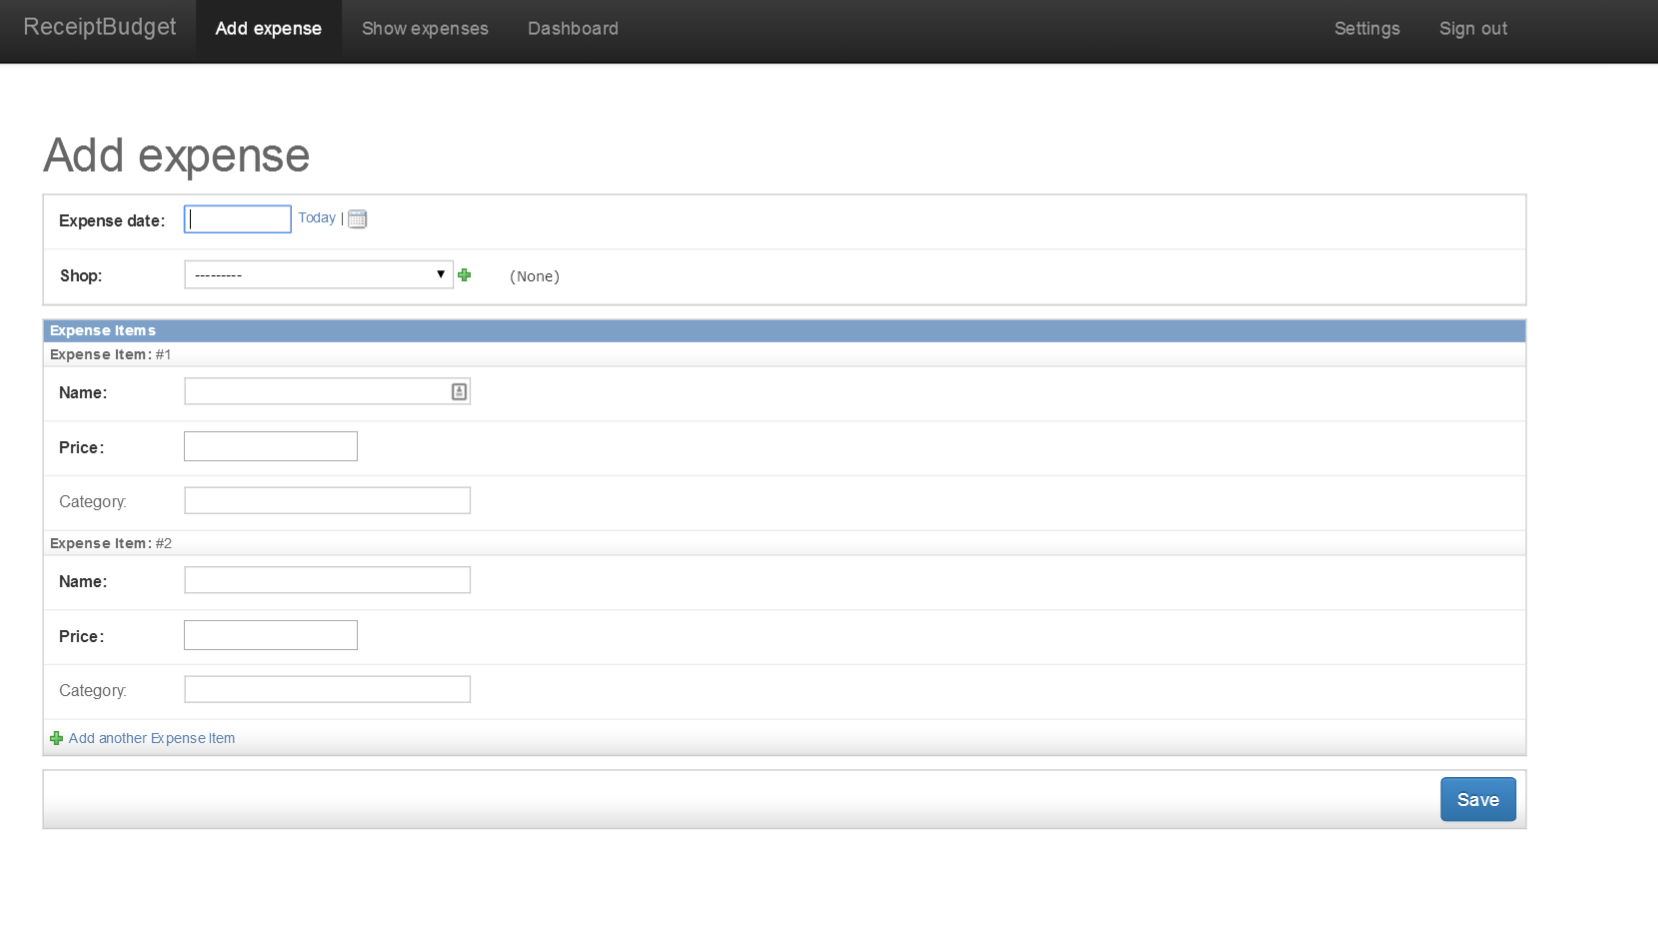
\includegraphics[width=\linewidth]{img/manual/manual_add.png}
\caption{\label{fig:manual_add}
The way to manually add a receipt}
\end{center}
\end{figure}

\begin{figure}[htdp]
\begin{center}
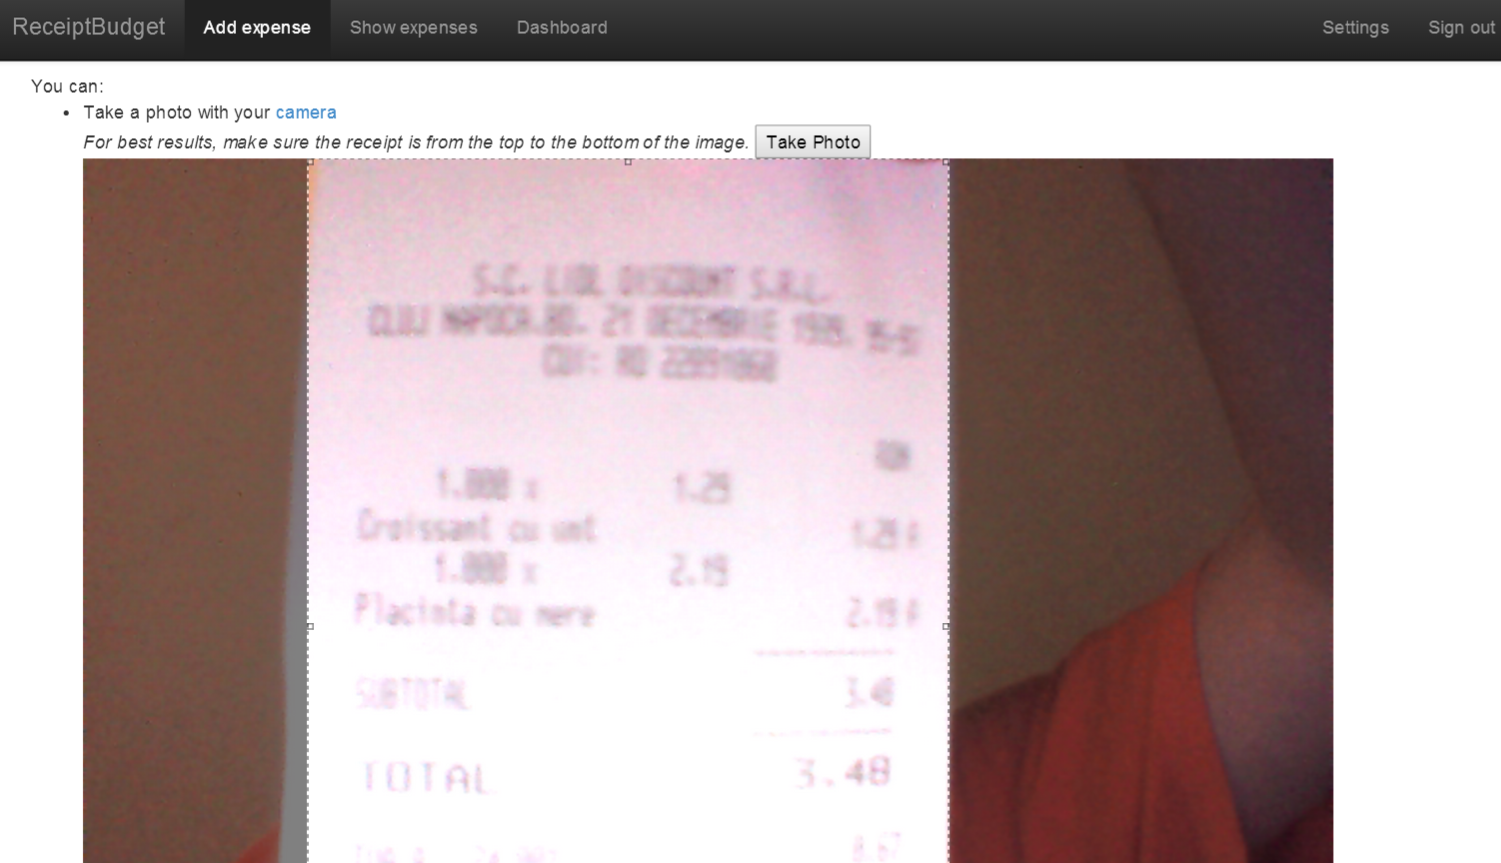
\includegraphics[width=\linewidth]{img/manual/webcam.png}
\caption{\label{fig:webcam}
Adding a receipt by taking a photo with a webcam}
\end{center}
\end{figure}

After the image has uploaded and the OCR engine has returned the extracted information, the user is shown the form from Figure \ref{fig:edit_expense} to edit the results in case there are any errors. After the errors are corrected, the user can save the expenses, or, if he wants, he can choose to discard them. 

\begin{figure}[htdp]
\begin{center}
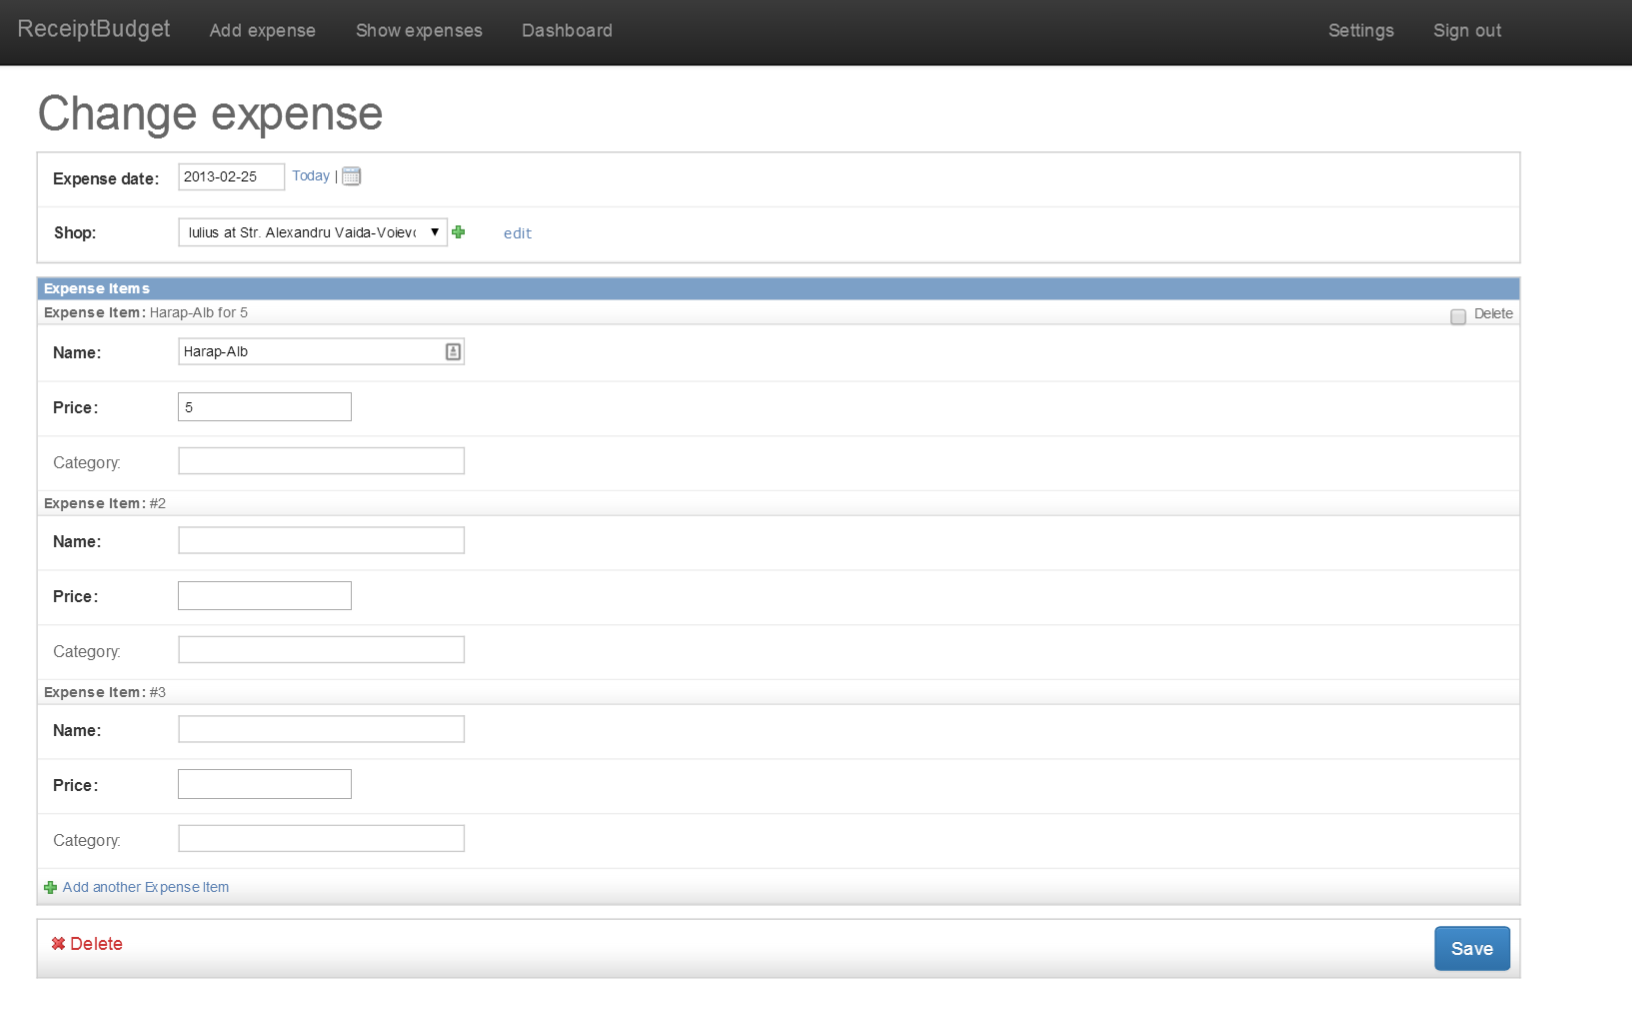
\includegraphics[width=\linewidth]{img/manual/edit_expense.png}
\caption{\label{fig:edit_expense}
Editing a receipt after OCR was performed on it to correct any errors}
\end{center}
\end{figure}

After the user has sufficient expenses in the system, they should visit the dashboard to see their spending pattern. The first visualization they can see on the dashboard is a heat map with all their expenses (Figure \ref{fig:all_map}). The stronger the color red is in an area, the more expenses have been made there. This map can be used to quickly identify hotspots where a lot of expenses are made.

\begin{figure}[htdp]
\begin{center}
\makebox[\textwidth][c]{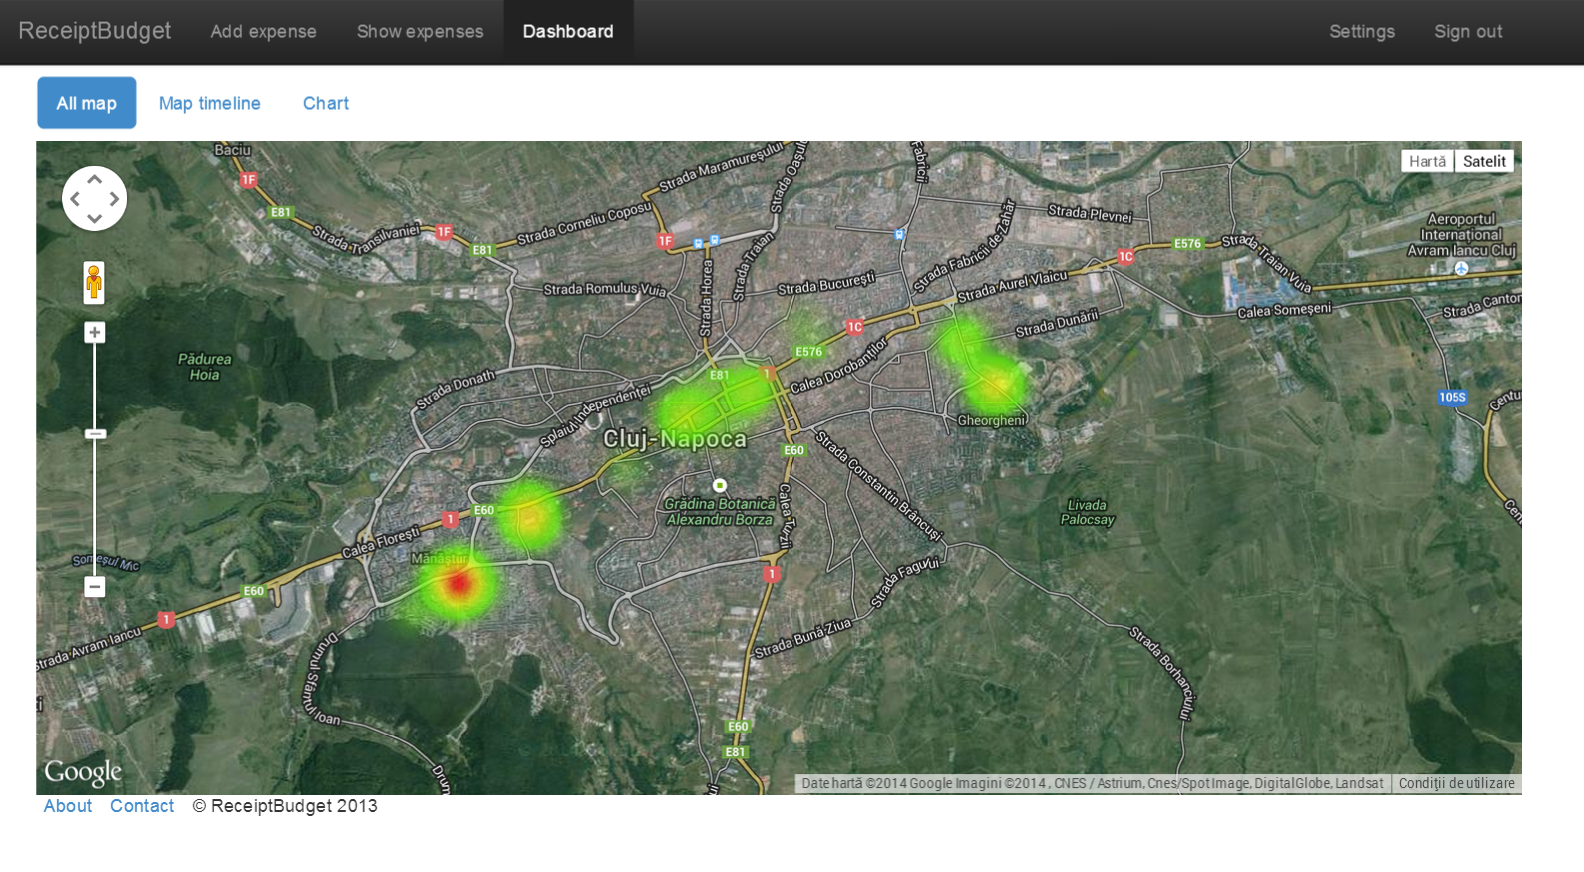
\includegraphics[width=1.2\linewidth]{img/manual/all_map.png}}
\caption{\label{fig:all_map}
The map part of the dashboard showing all expenses made}
\end{center}
\end{figure}

Another visualization is an animation of the way expenses are made each day, also plotted as a heat map (Figure \ref{fig:timeline}). Instead of showing all the expenses at the same time, this visualization breaks them down by day so that the user can see where they spent their money every day. This can be used to detect co-occurring expenses.

\begin{figure}[htdp]
\begin{center}
\makebox[\textwidth][c]{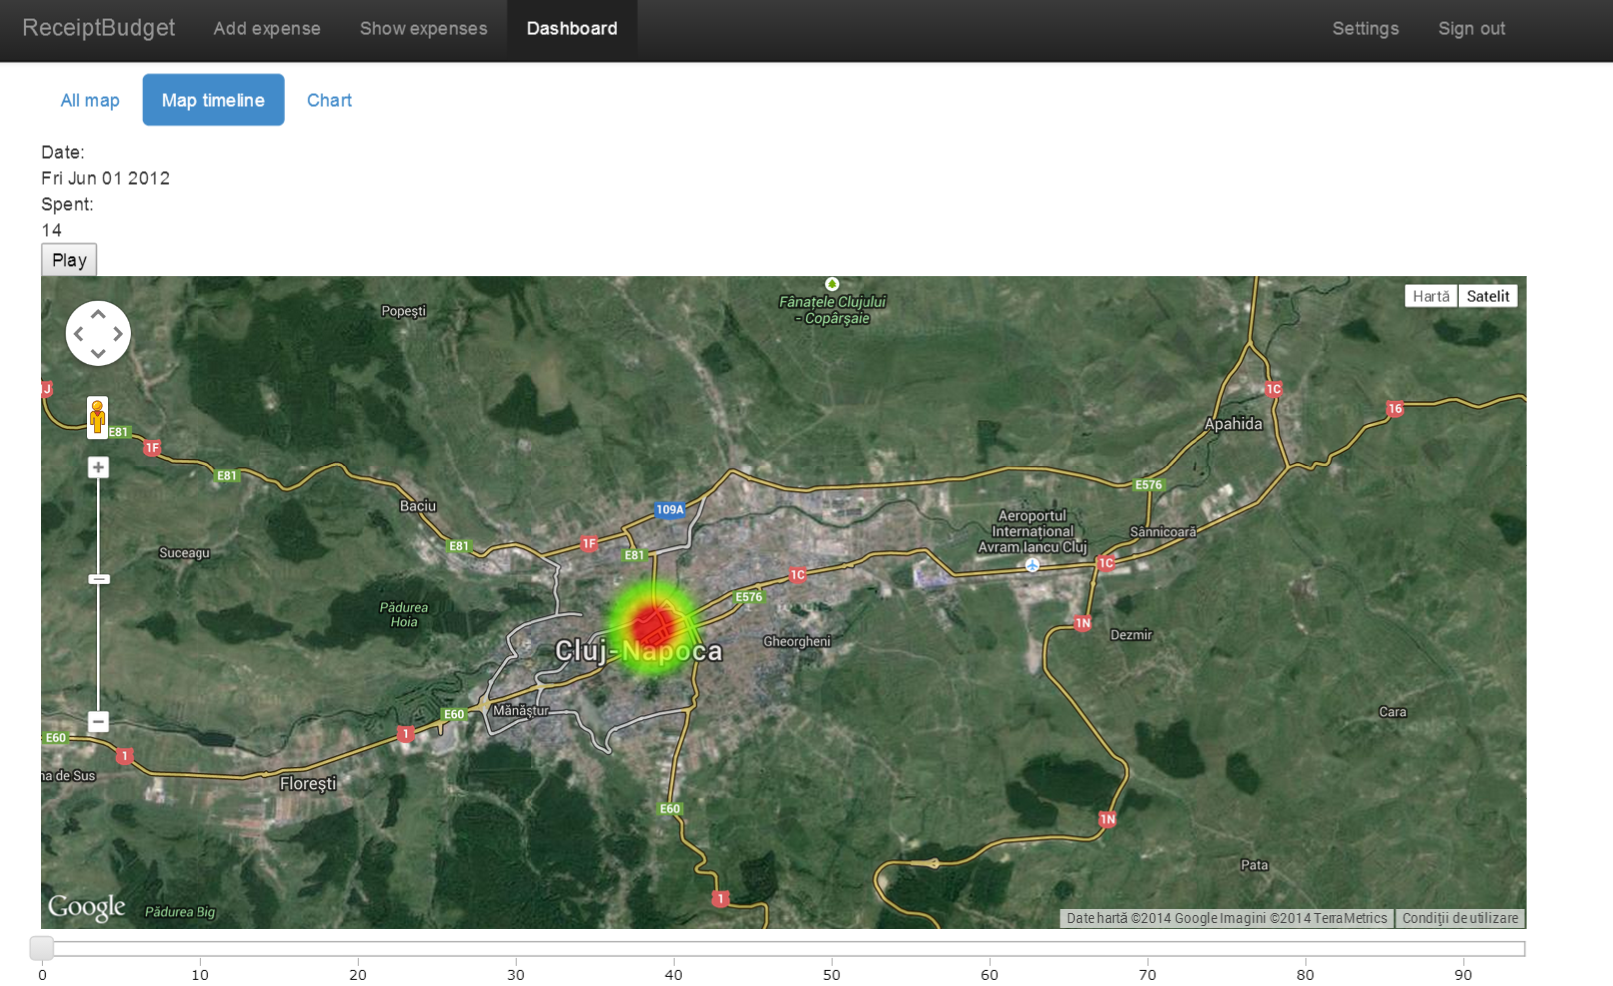
\includegraphics[width=1.2\linewidth]{img/manual/timeline.png}}
\caption{\label{fig:timeline}
A timeline view of the map, showing an animation of how many expenses were made each day}
\end{center}
\end{figure}

The final visualization is the proper dashboard, where there is a pie chart showing what shops was the money spent in, another pie chart showing how much money was spent in each month, a bar chart showing expense breakdown per days of the week, a graph showing the expenses over a range of dates and a table showing the selected expenses (Figures \ref{fig:top_dashboard} and \ref{fig:bottom_dashboard}). This dashboard is interactive and the user can manipulate each chart or graph to select a subset of the data and all the other graphs will be updated so that they show only information from the same subset. In this it is easy to see where a user has spent his money in the months of March, between 2012 and 2014, on weekends. 

\begin{figure}[htdp]
\begin{center}
\makebox[\textwidth][c]{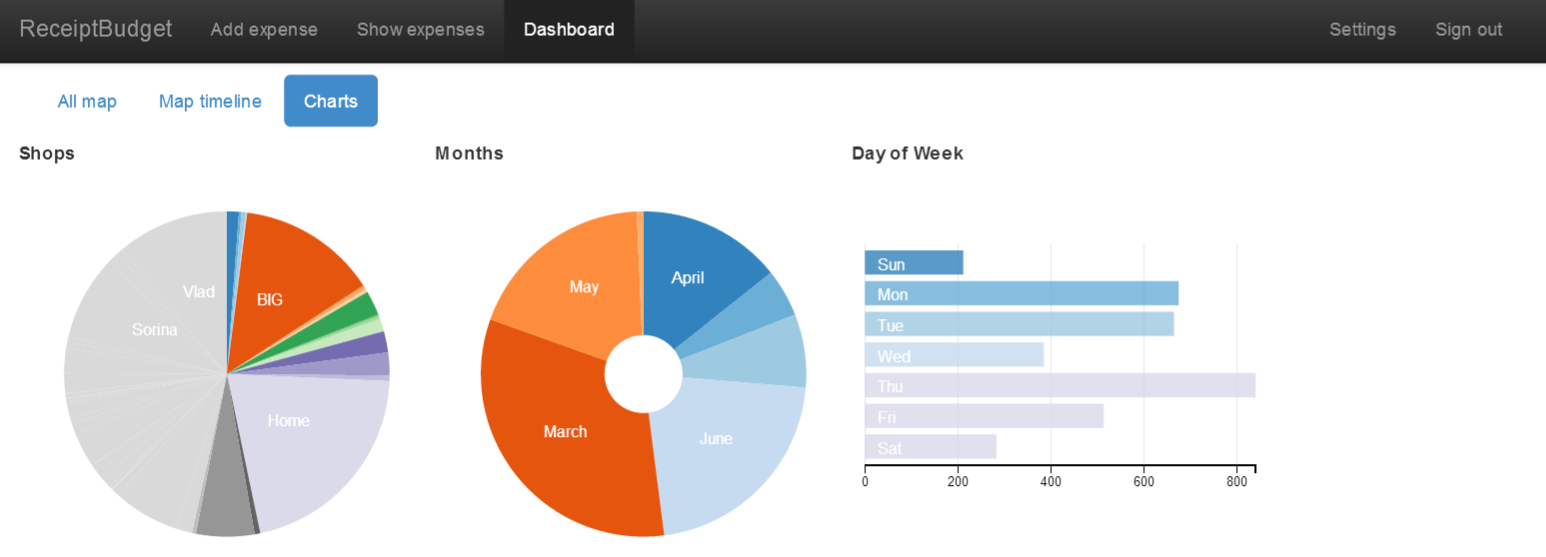
\includegraphics[width=1.2\linewidth]{img/manual/top_dashboard.png}}
\caption{\label{fig:top_dashboard}
The top part of dashboard where the user can filter his expenses}
\end{center}
\end{figure}


\begin{figure}[htdp]
\begin{center}
\makebox[\textwidth][c]{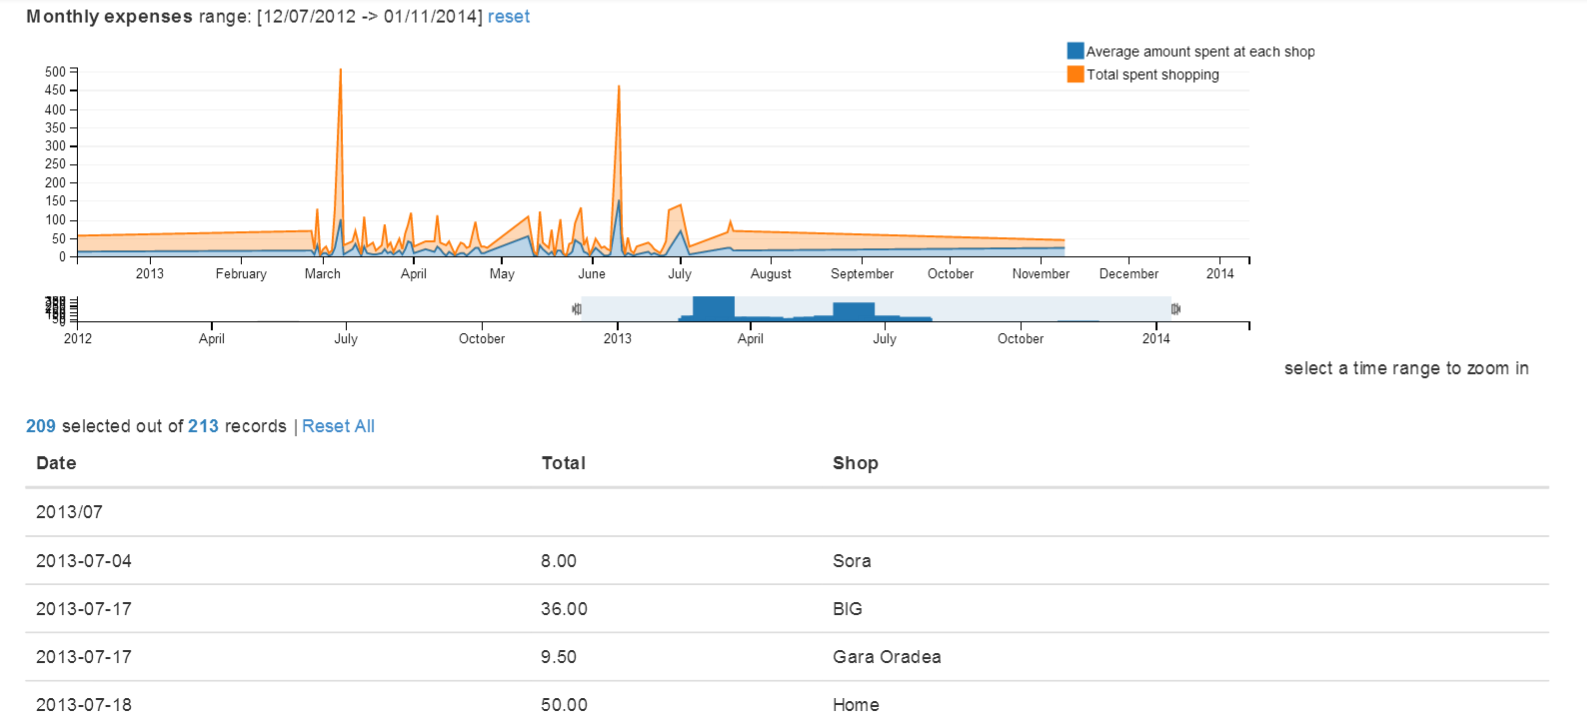
\includegraphics[width=1.2\linewidth]{img/manual/bottom_dashboard.png}}
\caption{\label{fig:bottom_dashboard}
The lower part of the dashboard}
\end{center}
\end{figure}
\section{Discussion}
This section analyzes our approaches and compares them to similar existing work.

\subsection{Analysis of the Proposed Approach}
In section \ref{sec:recog} we can see that using an SVM is a pretty good baseline for the character recognition problem, obtaining an average accuracy of 91\% with a RBF kernel. Using this type of kernel seems to seems to lead to slightly better results rather then just using a linear kernel, but not by more than 1-2\%. One explanation for this would be that the data is already high dimensional (400 dimensions) and the data points lie in sufficiently different parts so that the separating hyperplanes work effectively, without needing a projection into the infinite dimensional space offered by the RBF kernel. 

Using neural networks leads to much better results. When using the pretraining approach with two stacked autoencoders, the accuracy reaches about $95.6\% \pm 0.3 \% $. Switching to using two layers of linear rectified units, even without pretraining, leads to a further improvement of two percent in accuracy, reaching $ 97.9\% \pm 1.2\% $. The 3 layered network has fewer neurons than the two layered one, but it still manages to give almost the same level of accuracy, $ 97.5\% \pm 1.7\% $, showing the advantages of using more layers, even if they are narrower. The best results are obtained using the the four layered neural network, which gives an accuracy of $ 98.5\% \pm 0.2\% $. 

In the case of the character segmentation, the values of the parameter didn't matter that much. The difference between the best and the worst result was about 0.2. The number of features had the most influence, of $ 0.1\% $, on the F1 score, while the number of trees influenced it only by 0.01. The highest average was obtained for the values of 250 trees in the forest and 40 features chosen at each split, giving an F1 score of $ 87.936\% \pm 0.445$ on the validation set and a score of $ 91.99\% $ on the test set.  

This seems to indicate that the number of features that are chosen at each split point is a more important parameter for random forests, while the number of trees used in the forest doesn't vary the results so much. This is in line with the theoretical basis of random forests\cite{breiman2001random}, which suggest that random forests are somewhat sensitive to the number of features used in them. 


% todo
If we look at the confusion matrix for the character recognition problem, computed for the whole data set, we can see that one of the most often made mistakes are:
\begin{itemize}
\item confusing , with . - 28 times
\item confusing . with , - 12 times
\item confusing O with 0 - 24 times
\item confusing 0 with O - 15 times
\item confusing 0 with o - 3 times
\item confusing l with I - 6 times
\item confusing I with T - 5 times
\item confusing I with 1 - 4 times
\item confusing 1 with I - 4 times
\end{itemize} 

These mistakes are easy to make: a comma and a period are very similar, especially in a noisy, low resolution environment. The lower and upper case letters O are again very similar to the digit 0, on some receipts there being no distinction between O and 0, only the context in which they are used. For monospace fonts, which some receipts use, the lack of difference between l, I, 1 is a well known problem, which is why many design books and human computer interaction studies recommend using other fonts\cite{chaparro2006examining}. 

If we look at the confusion matrix for the character segmentation problem, we see that it makes the mistake of not predicting a split more often than it does the opposite, so the model is more specific, rather then sensitive. 

Specifity and sensitivity can be computed as\cite{Fawcett_2006}

\[
    \text{sensitivity} = \frac{\text{true positives}}{\text{all positives}} = \frac{2546}{2546+363} = 87.52 \%
\]
\[
    \text{specificity} = \frac{\text{true negatives}}{\text{all negatives}} = \frac{4556}{4556+255} =  94.70 \%
\]

Another good evaluation measure is the \textit{Area unde the ROC curve} (AUC)\cite{Fawcett_2006}. The \textit{ROC} (Receiver Operating Characteristic) curve is a plot of \textit{sensitivity} versus (1 - \textit{specificity}). Usually they are constructed from classifiers that instead of a label, return a score that can be converted into a label by thresholding. In the case of classifiers that return the class directly, the ROC curve has only one point, from where the AUC measure can be computed. 

In our case, the AUC is 0.911, as computed from the graph in figure \ref{fig:roc}. 


\begin{figure}[h!]
\begin{center}
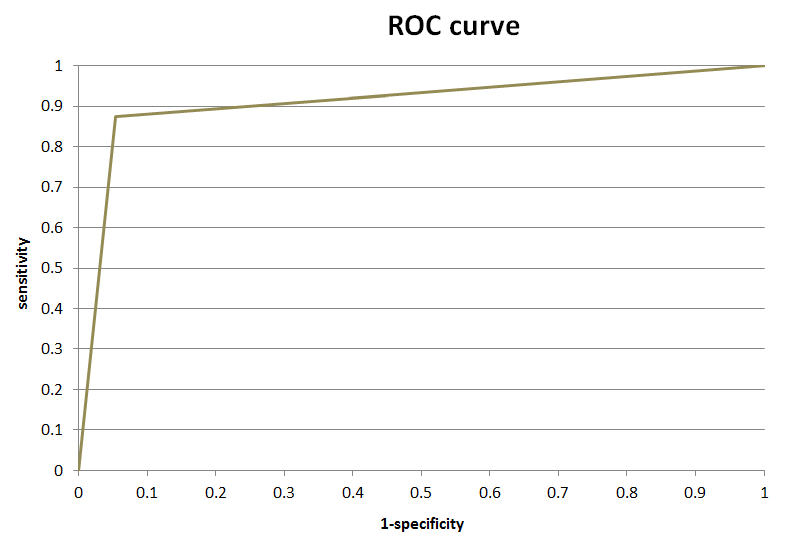
\includegraphics[width=0.7\columnwidth]{img/roc.png}
\caption{\label{fig:roc}
ROC curve for the character segmentation problem}
\end{center}
\end{figure}

\subsection{Comparison to Related Work}
If we compare the results of the character recognition problem with the ones obtained on the MNIST dataset\cite{lecun1998mnist}, we see that our error rates are much higher: around 1.5\% versus 0.23\% (obtained by using a deep and wide neural network on MNIST). There are several possible explanations for this. One is that MNIST has only ten classes (corresponding to the ten digits), so it is much easier for a classifier to assign the correct class to a data point, compared to our dataset, which has 74 distinct classes, of which many are similar (the digit 0 and the letters o and O, the digit 1 and the letter l). Another factor that makes MNIST easier to solve is the fact that it has 70000 datapoints in total, while our dataset contains only 7045 data points. This almost ten fold difference has a great contribution to the ability of the classifier to generalize. Even on the MNIST dataset, adding more data is beneficial, as show by Ciresan et al.\cite{Cire_an_2010}, who obtained one of the best results on MNIST by augmenting the dataset with artificial data generated by transforming the existing digits. Also, one of the state-of-the-art neural network that obtained these results on MNIST had 9 layers of 1000 neurons each, so it has a much greater representational power than our 4 layered network having 2000 neurons in total. 

The results obtained in \cite{kahraman2003license} and \cite{Franc_2005} for the character segmentation problem are a bit better than our results: 94.5\% and 96.7\% accuracy, compared to our 91.9\%. The difference between the two problems is that in their papers the number of characters in a licence plate is known and fixed, while lines in a receipt have varying lenghts. This prior knowledge used by them can explain the difference in results. 

The paper by Janssen\cite{janssen2012receipts2go} deals with OCR on receipts, but they don't train the OCR engine for receipts, they just present a new approach for image normalization. In contrast, our approach improves the accuracy of the OCR engine by focusing on the character segmentation and recognition problem. 

The best free OCR engine on the market, Tesseract, performs quite poorly. On the receipt seen in Figure \ref{fig:orig_image}, it produces the following text output:

\begin{minipage}{0.5\linewidth}
\begin{verbatim}
S.C. HRTIHH 5.9.
ELUJ NHPUCH. STR. BUCEGI. NR. 19

9.9.1. 99 11735629
RUN
1.999 x 3.19
BRTISTE N9Z.CLHS|C3S 3.19 9
1.999 x 2.59
STICKLETTI CHRTUF 99 2.59 9
9.399 x 7.99
HHNDHRINE 3.12 H
9.446 x 7.99
99511 3.56 9
1.999 x 11.29
SHLHH C959 USCHT 299 11.29 9
SUBTUTHL 23.5?
SUBTUTRL _____ ‘-29:99
TUTHL 23.57
TUH 9 24.992 4.55 9
TUTHL 23.5?
Nunerar 199.99
REST ?E.43

Carrefour ua nultuneste
si ua doreste

0 21 buna1
11*#9111¥¥*¥¥¥#*¥¥**1¥¥¥¥¥¥¥
TEL: 9374.294.B33
FHX: 9374.294.934
TELUERDE 9999.9B99.92
X1441111¥*¥¥*¥¥¥¥¥%%*¥¥*¥¥¥¥

99:91 PS:3 95:24 TR:11591

BF. 944 DHTH:23/94/2913 9RH:29~22-59
E1. CJ9563953455
BONFISCHL
\end{verbatim}
\captionof{figure}{Output produced by Tesseract}
\end{minipage}
\begin{minipage}{0.5\linewidth}
\begin{verbatim}
S.C.   ARTIMA  S.A.
CLUJMAPOCA,  STR.  BUCEGI,  NR. 19
C  .U.1,R O1   1735628
RON
1.000  x  3,19
BATISTE NAZ.CLASIC3S 3,19%
1,000x   2,50
STICNLETTI  CARTOF  80   2,50  A
0,390  x  7,99
MANDARINE   3,12A
0,446  x  7,99
R0SI 3,56  A
1.000  x 11,20
SALANIASAOSCAT  290  11,20A
SUBTOTAL   23,57
SUBTOTAL 23,57
TOTAL   27,57
IVA   A 24,00%   4,56
IOTAL   23,57
Numera8  100,00
REST   76,43
Ca8-8-efoLr   ua   multLxmeste
Sl  0B O0tR8st8
O   21 Dt   A8!
****************************
TEL:  0I74.204.833
FAX:   0374.204.834
tELUERDE  0800.0800.02
****************************
MG:81  PS:3  CS:24   TR:11581
BF.   844   DATA:23/04/2013 ORA:20-22-58
R CJ0563053455
B OB  F S  CA L
\end{verbatim}
\captionof{figure}{Output produced by the OCR engine of ReceiptBudget}
\end{minipage}

By comparing to the output of ReceiptBudget, it can be seen that the latter is much better, even though it is not yet perfect. Tesseract completely fails to recognize the shop name, the date and the CUI, the address is only partially recognized and most of the bought items are unrecognizable. 
